\documentclass[twocolumn,a4j]{jsarticle}
\setlength{\topmargin}{-20.4cm}
\setlength{\oddsidemargin}{-10.4mm}
\setlength{\evensidemargin}{-10.4mm}
\setlength{\textwidth}{18cm}
\setlength{\textheight}{26cm}

\usepackage[top=15truemm,bottom=25truemm,left=15truemm,right=15truemm]{geometry}
\usepackage[latin1]{inputenc}
\usepackage{amsmath}
\usepackage{amsfonts}
\usepackage{amssymb}
\usepackage[dvipdfmx]{graphicx}
\usepackage[dvipdfmx]{color}
\usepackage{listings}
\usepackage{listings,jvlisting}
\usepackage{geometry}
\usepackage{framed}
\usepackage{color}
\usepackage[dvipdfmx]{hyperref}
\usepackage{ascmac}
\usepackage{enumerate}
\usepackage{tabularx}
\usepackage{cancel}
\usepackage{scalefnt}

\renewcommand{\figurename}{Fig.}
\renewcommand{\tablename}{Table }

\lstset{
basicstyle={\ttfamily},
identifierstyle={\small},
commentstyle={\smallitshape},
keywordstyle={\small\bfseries},
ndkeywordstyle={\small},
stringstyle={\small\ttfamily},
frame={tb},
breaklines=true,
columns=[l]{fullflexible},
xrightmargin=0zw,
xleftmargin=3zw,
numberstyle={\scriptsize},
stepnumber=1,
numbersep=1zw,
lineskip=-0.5ex
}

\makeatletter
\def\@maketitle
{
\begin{center}
{\LARGE \@title \par}
\end{center}
\begin{flushright}
{\large 報告書 NO.08 - 2\quad\@date\quad\@author}
\end{flushright}
\par\vskip 1.5em
}
\makeatother

\setcounter{tocdepth}{3}

\author{来代 勝胤}
\title{令和3年度 12月 第2週 報告書}
\date{2021/12/9}

\begin{document}
\columnseprule=0.1mm

\maketitle
\section{Raw data}
\subsection{0 deg}
\begin{figure}[htbp]
    \footnotesize
    \begin{center}
        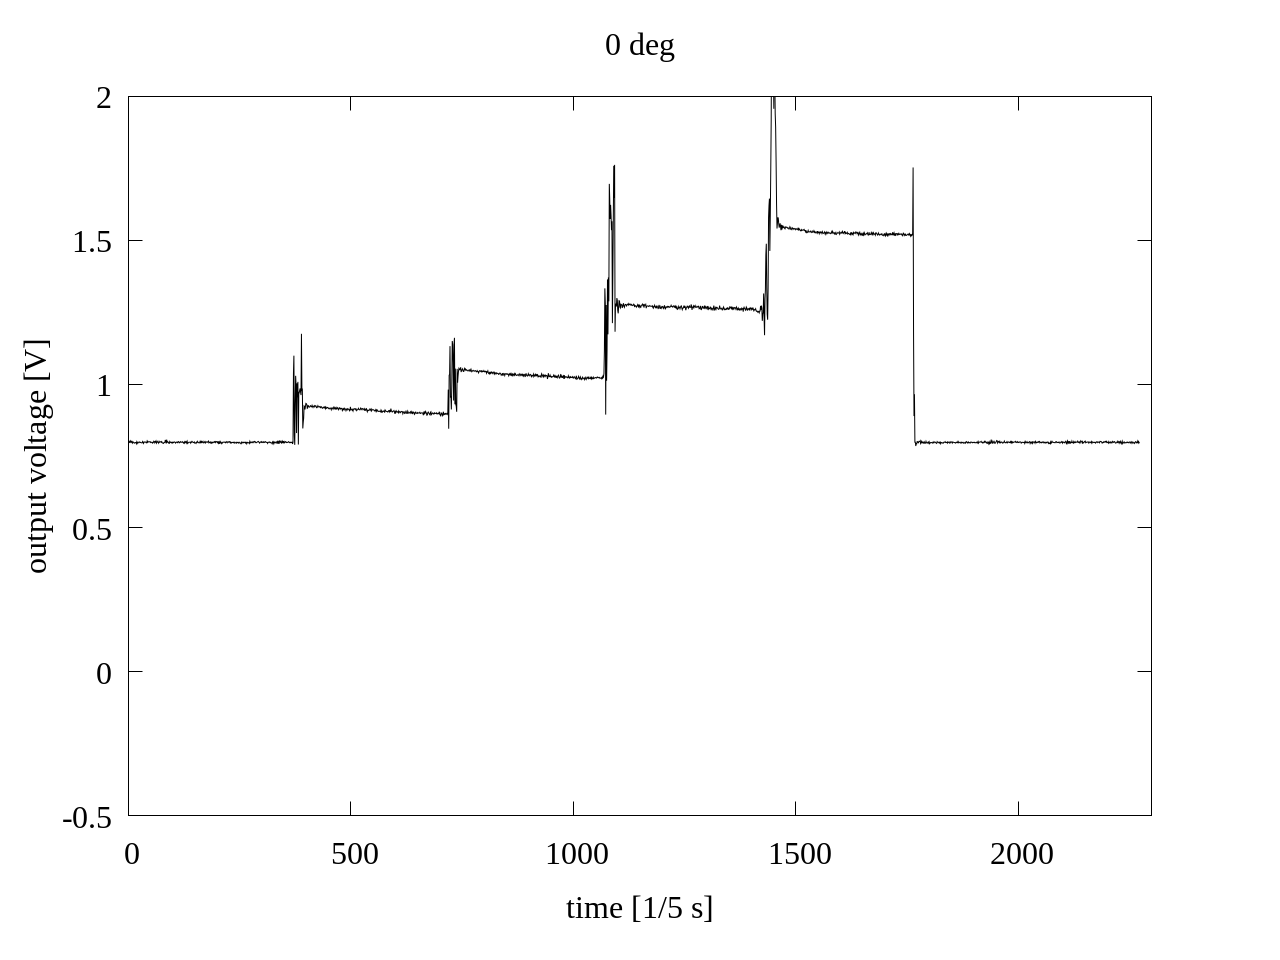
\includegraphics[width=88mm]{../images/reverse/0_loadcell.png}
        \caption{Result of loadcell voltage}
        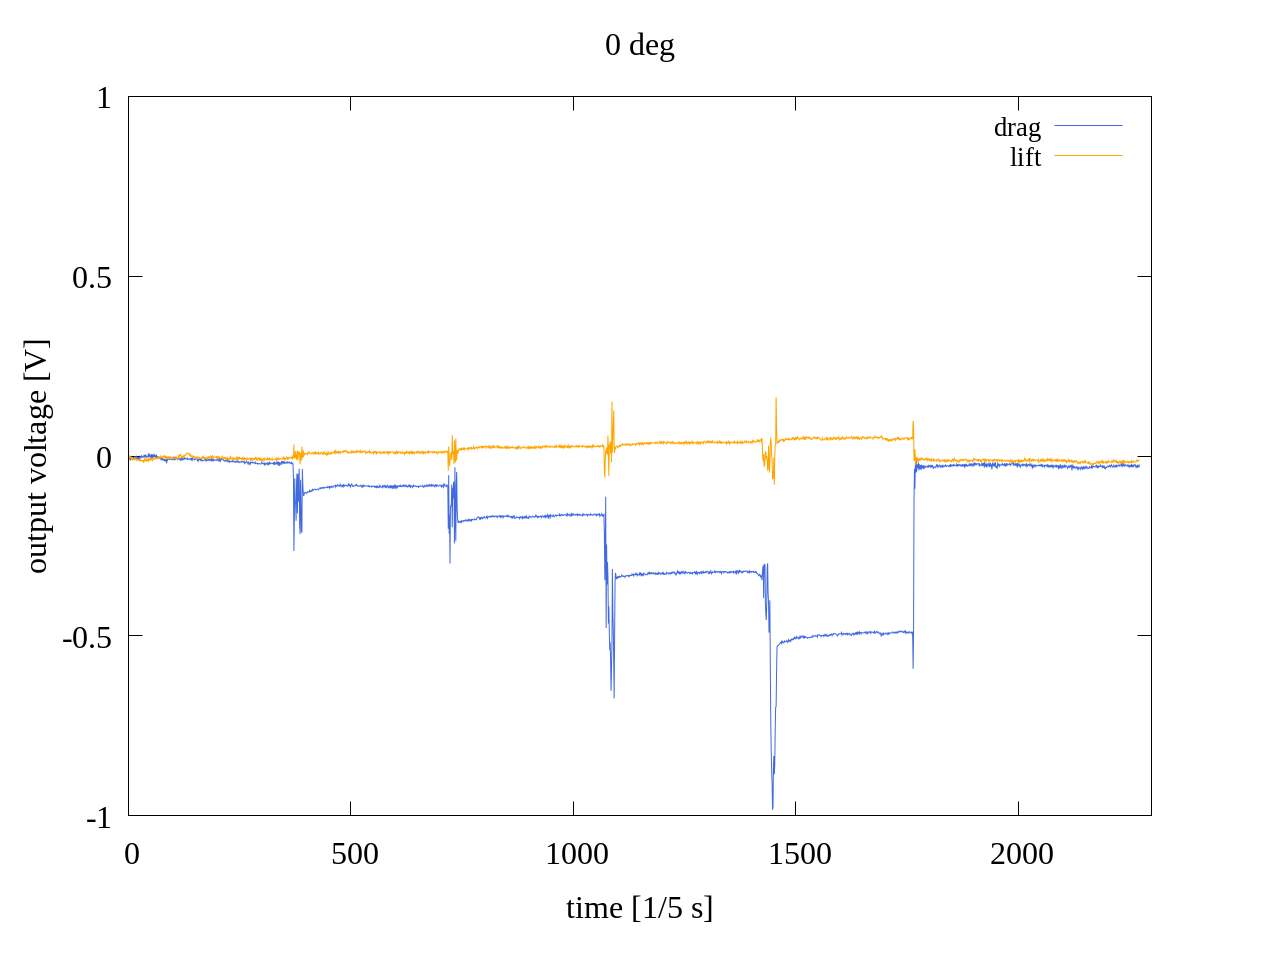
\includegraphics[width=88mm]{../images/reverse/0_strainsensor.png}
        \caption{Result of strainsensor voltage}
    \end{center}
\end{figure}

\newpage
\subsection{15 deg}
\begin{figure}[htbp]
    \footnotesize
    \begin{center}
        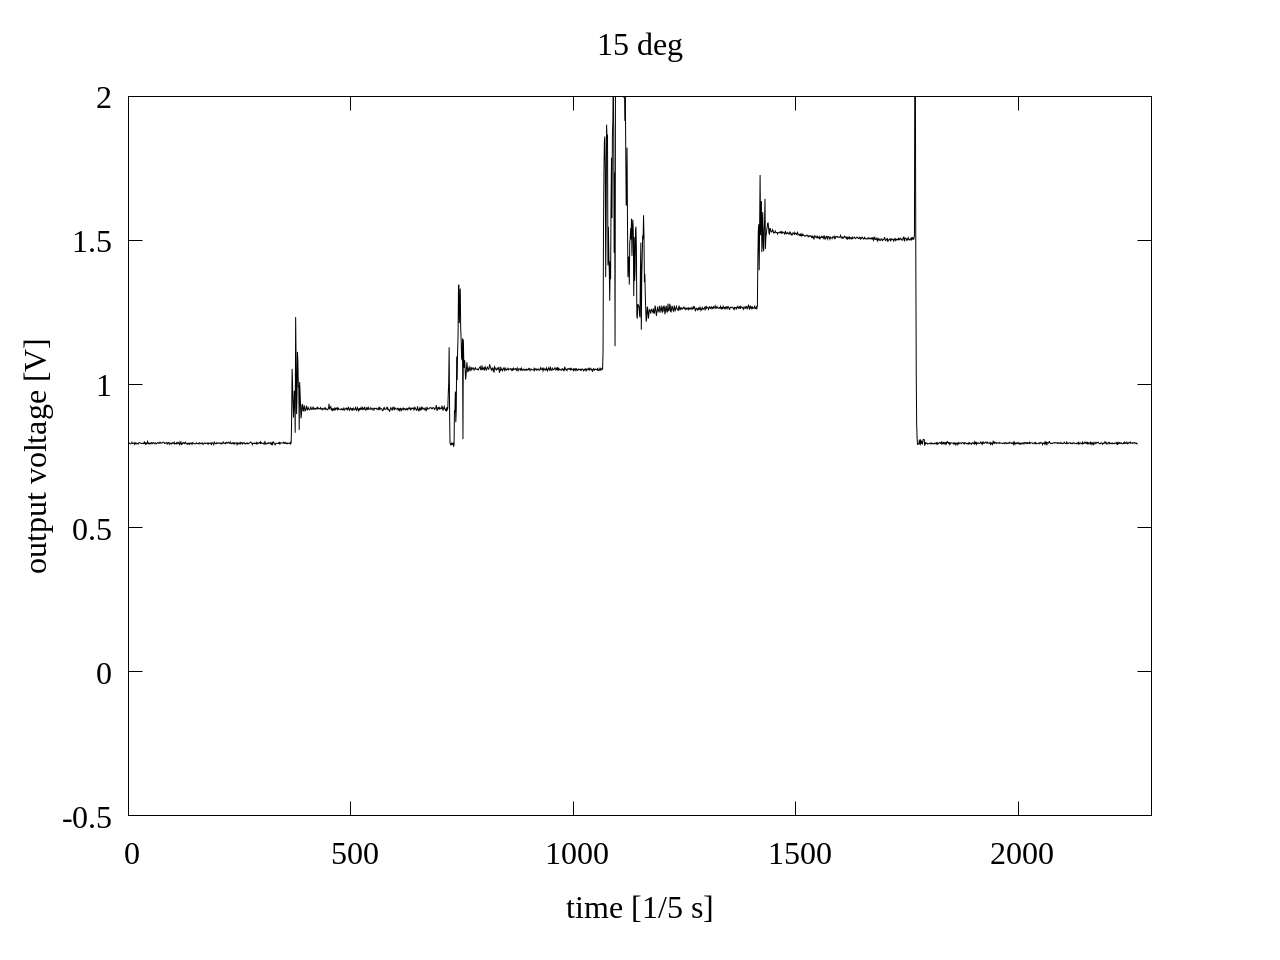
\includegraphics[width=88mm]{../images/reverse/15_loadcell.png}
        \caption{Result of loadcell voltage}
        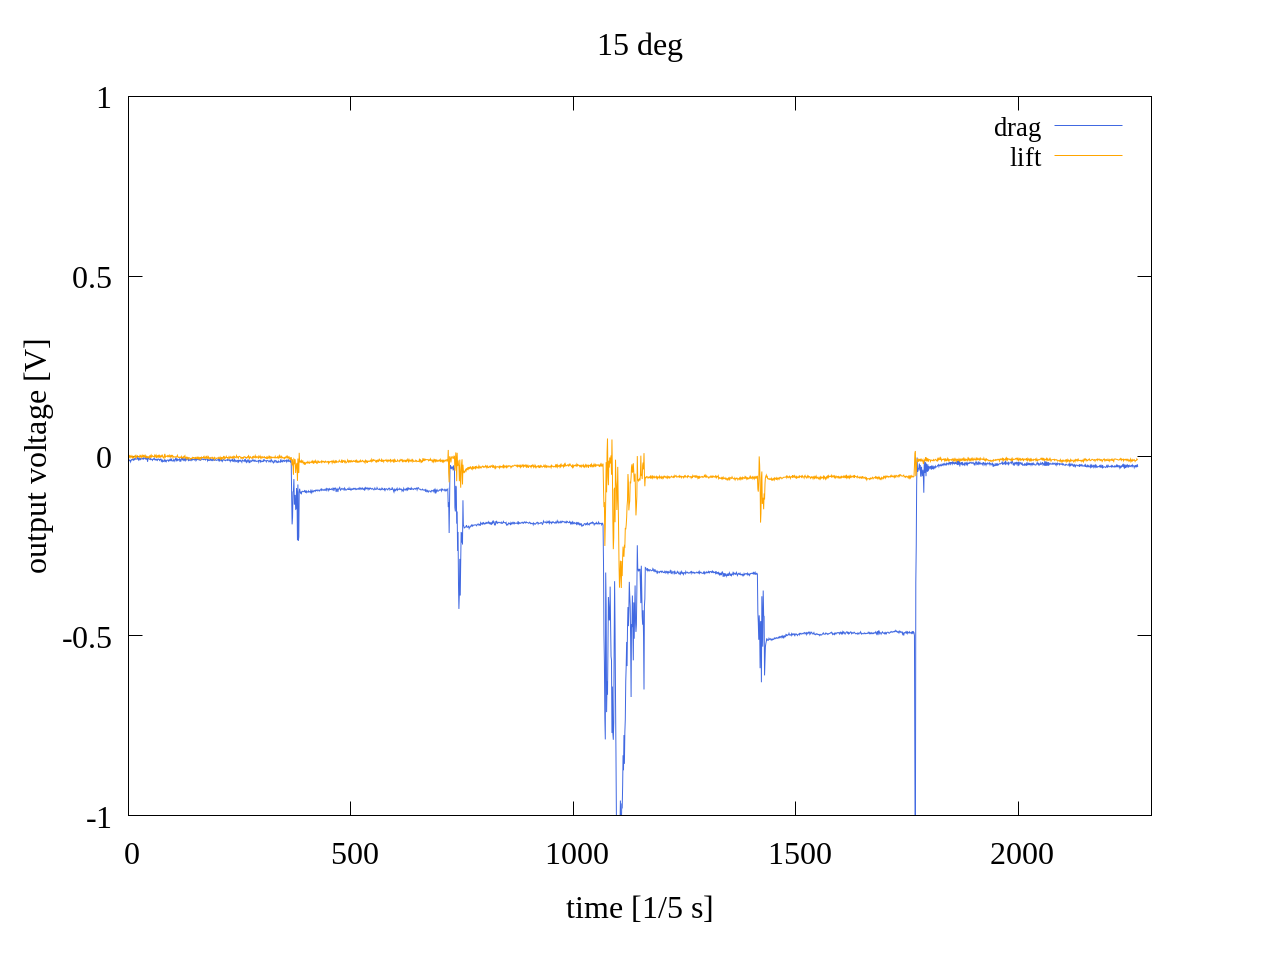
\includegraphics[width=88mm]{../images/reverse/15_strainsensor.png}
        \caption{Result of strainsensor voltage}
    \end{center}
\end{figure}

\newpage
\subsection{30 deg}
\begin{figure}[htbp]
    \footnotesize
    \begin{center}
        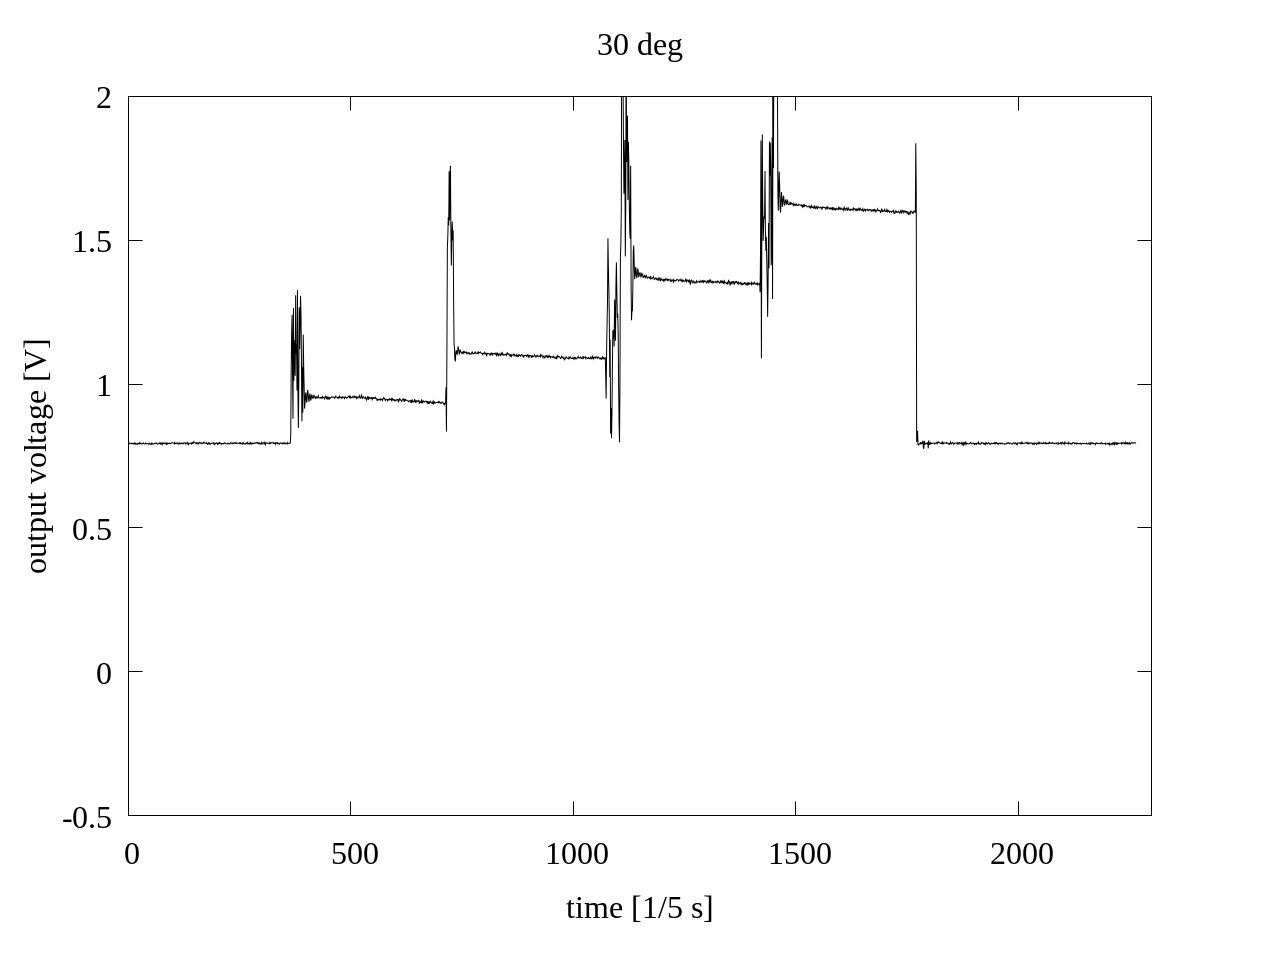
\includegraphics[width=88mm]{../images/reverse/30_loadcell.png}
        \caption{Result of loadcell voltage}
        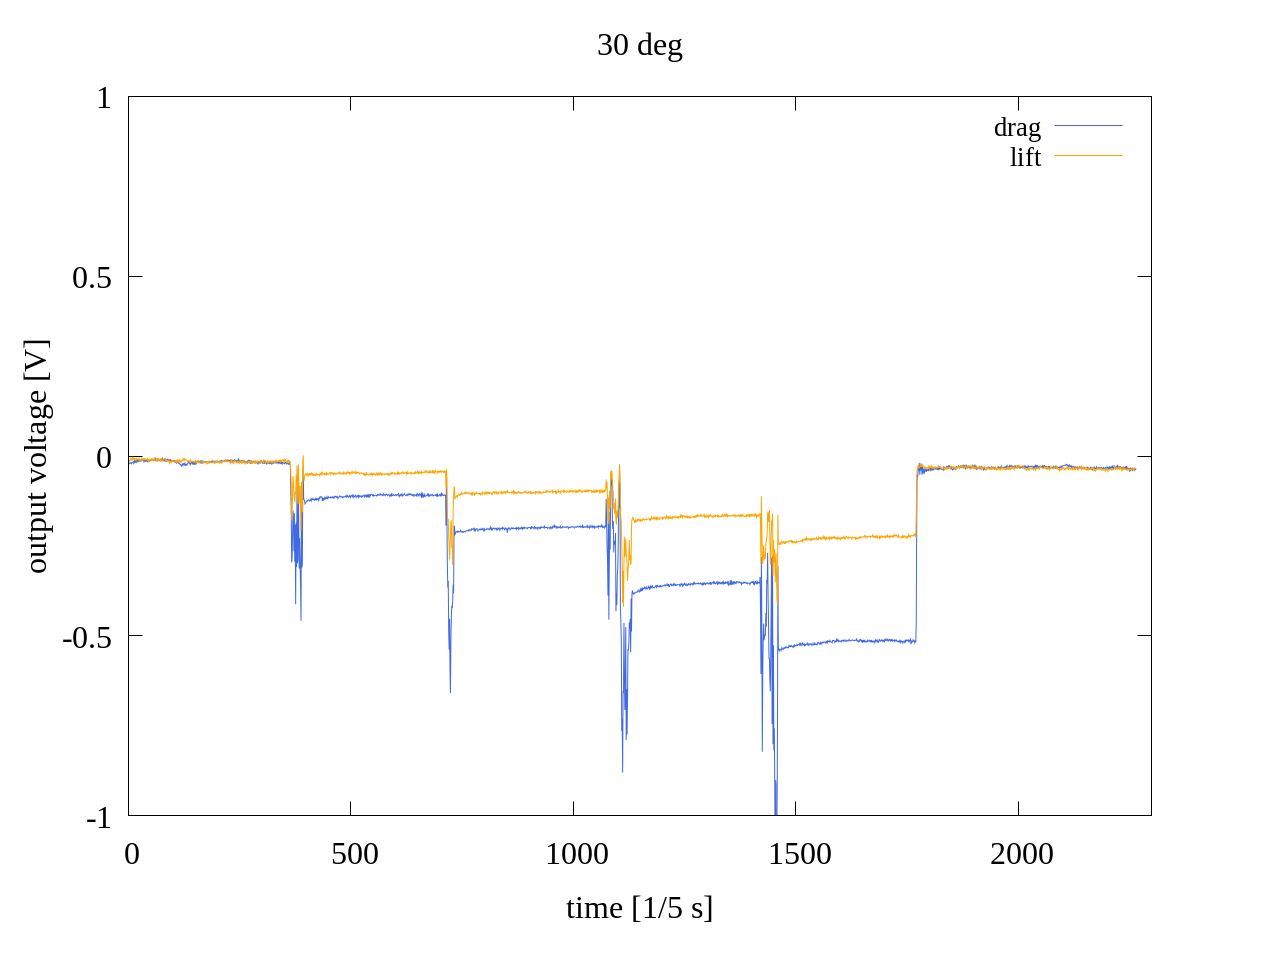
\includegraphics[width=88mm]{../images/reverse/30_strainsensor.png}
        \caption{Result of strainsensor voltage}
    \end{center}
\end{figure}

\newpage
\subsection{45 deg}
\begin{figure}[htbp]
    \footnotesize
    \begin{center}
        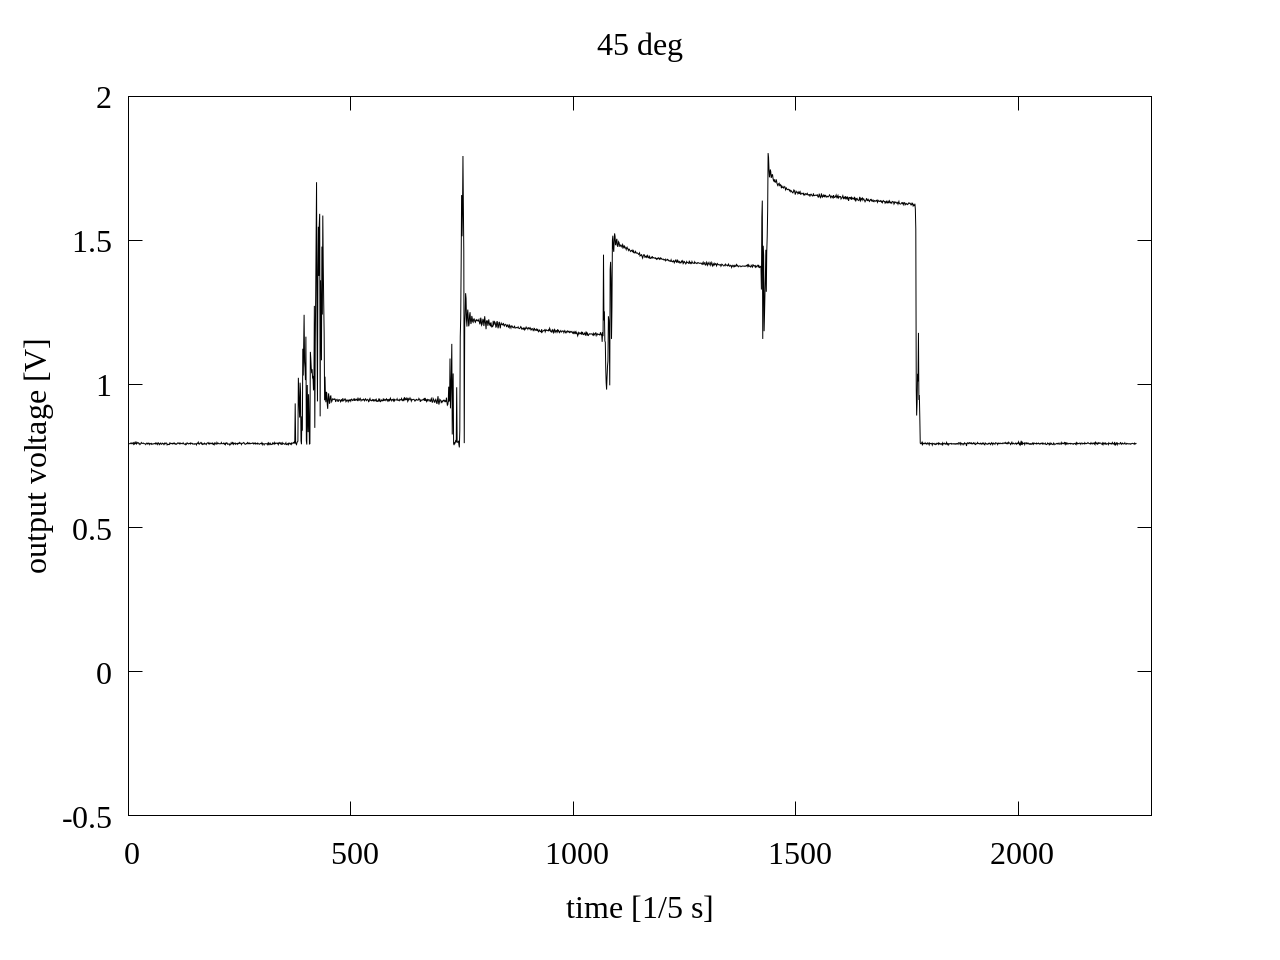
\includegraphics[width=88mm]{../images/reverse/45_loadcell.png}
        \caption{Result of loadcell voltage}
        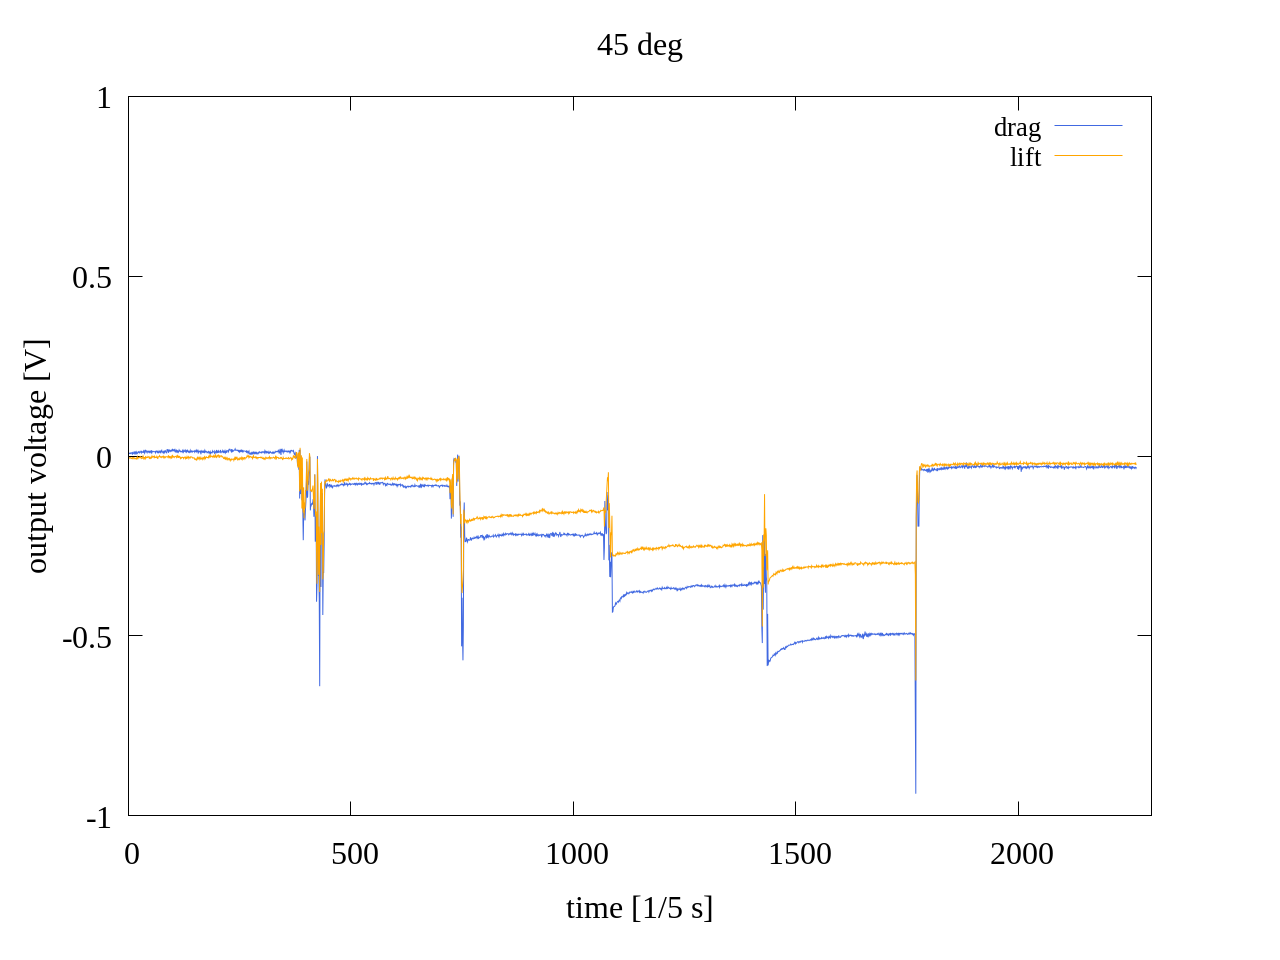
\includegraphics[width=88mm]{../images/reverse/45_strainsensor.png}
        \caption{Result of strainsensor voltage}
    \end{center}
\end{figure}

\newpage
\subsection{60 deg}
\begin{figure}[htbp]
    \footnotesize
    \begin{center}
        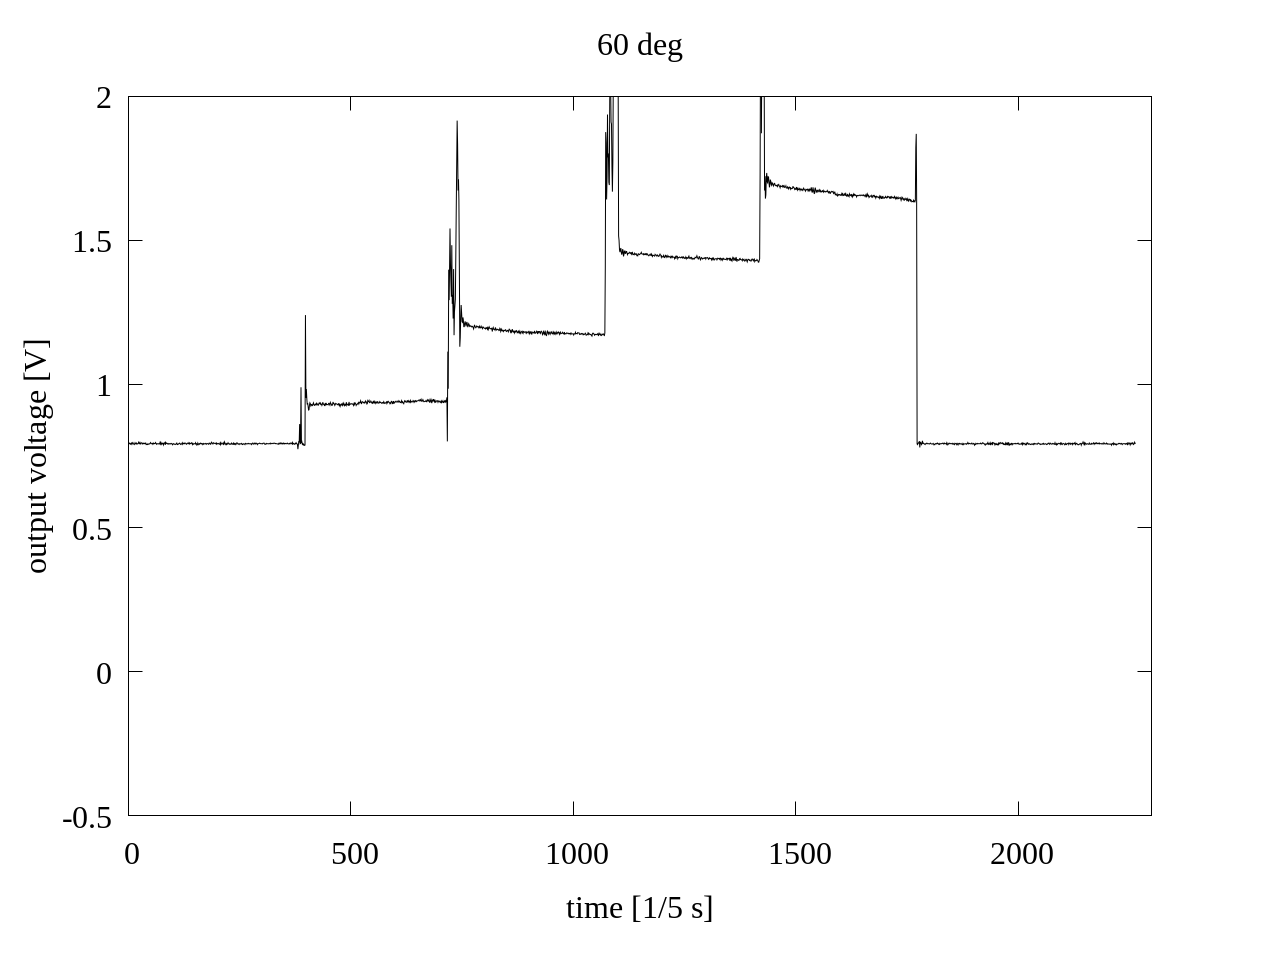
\includegraphics[width=88mm]{../images/reverse/60_loadcell.png}
        \caption{Result of loadcell voltage}
        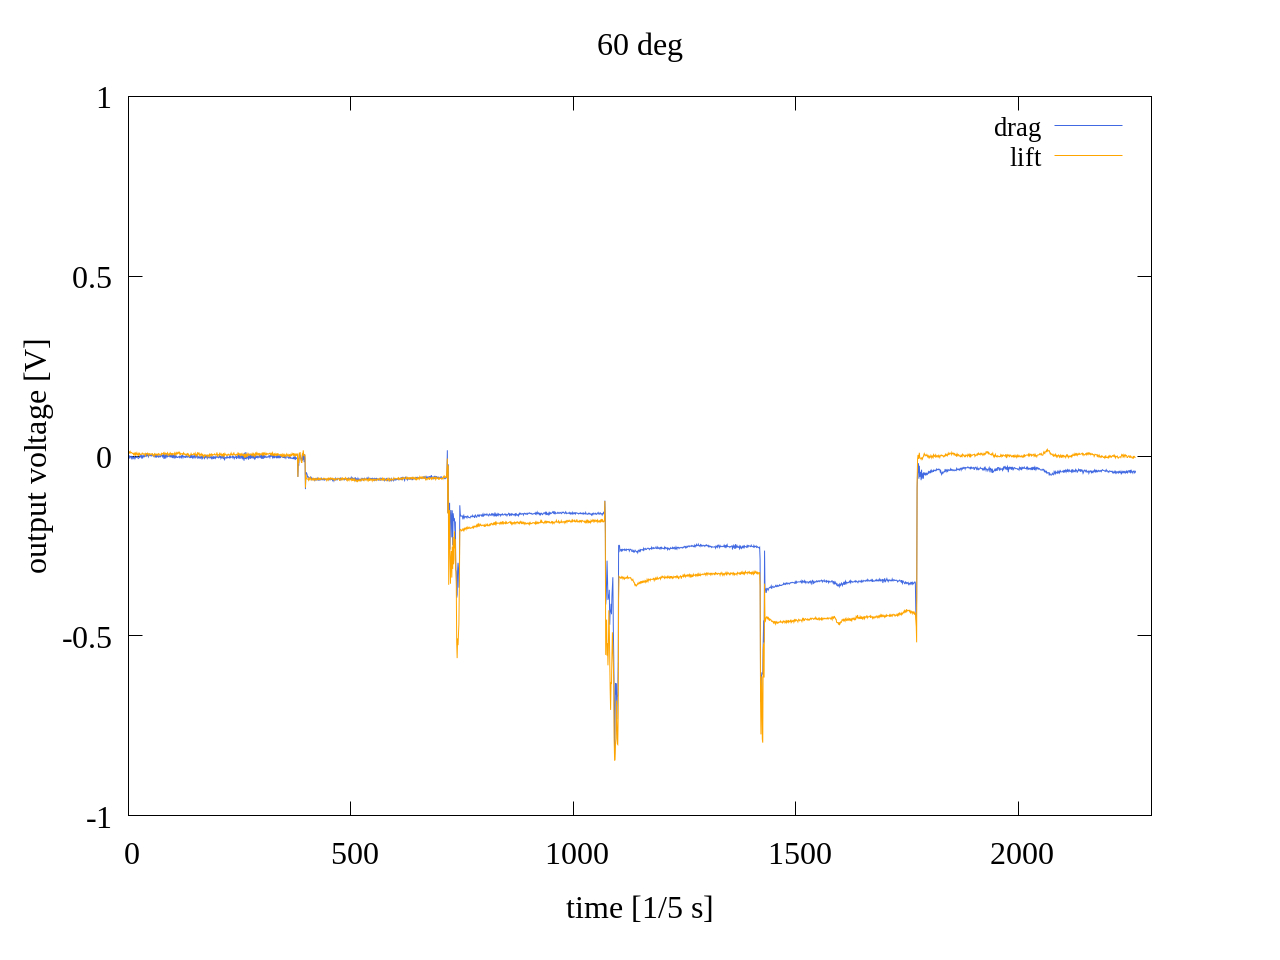
\includegraphics[width=88mm]{../images/reverse/60_strainsensor.png}
        \caption{Result of strainsensor voltage}
    \end{center}
\end{figure}

\newpage
\subsection{75 deg}
\begin{figure}[htbp]
    \footnotesize
    \begin{center}
        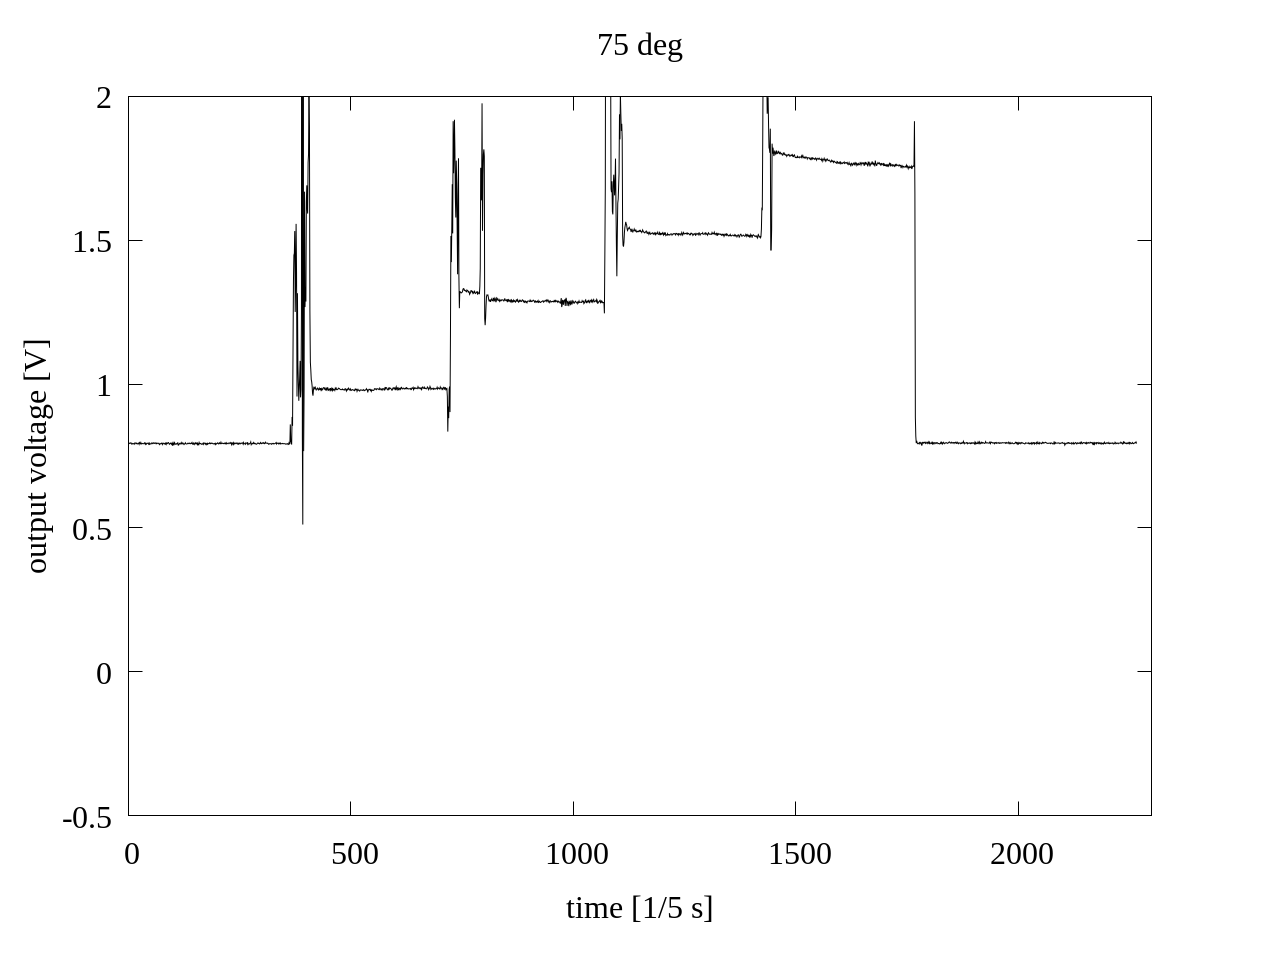
\includegraphics[width=88mm]{../images/reverse/75_loadcell.png}
        \caption{Result of loadcell voltage}
        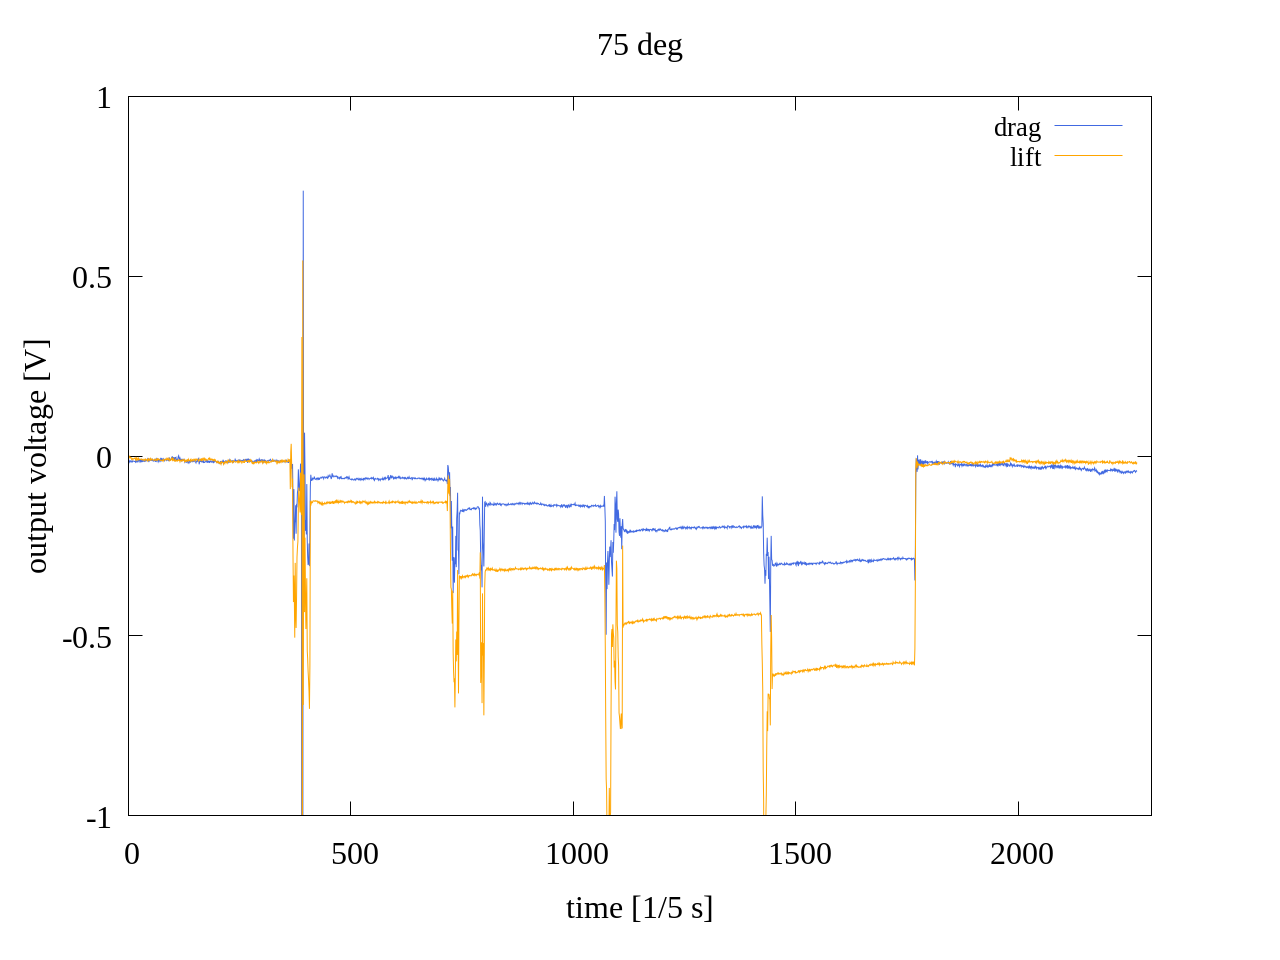
\includegraphics[width=88mm]{../images/reverse/75_strainsensor.png}
        \caption{Result of strainsensor voltage}
    \end{center}
\end{figure}

\newpage
\subsection{90 deg}
\begin{figure}[htbp]
    \footnotesize
    \begin{center}
        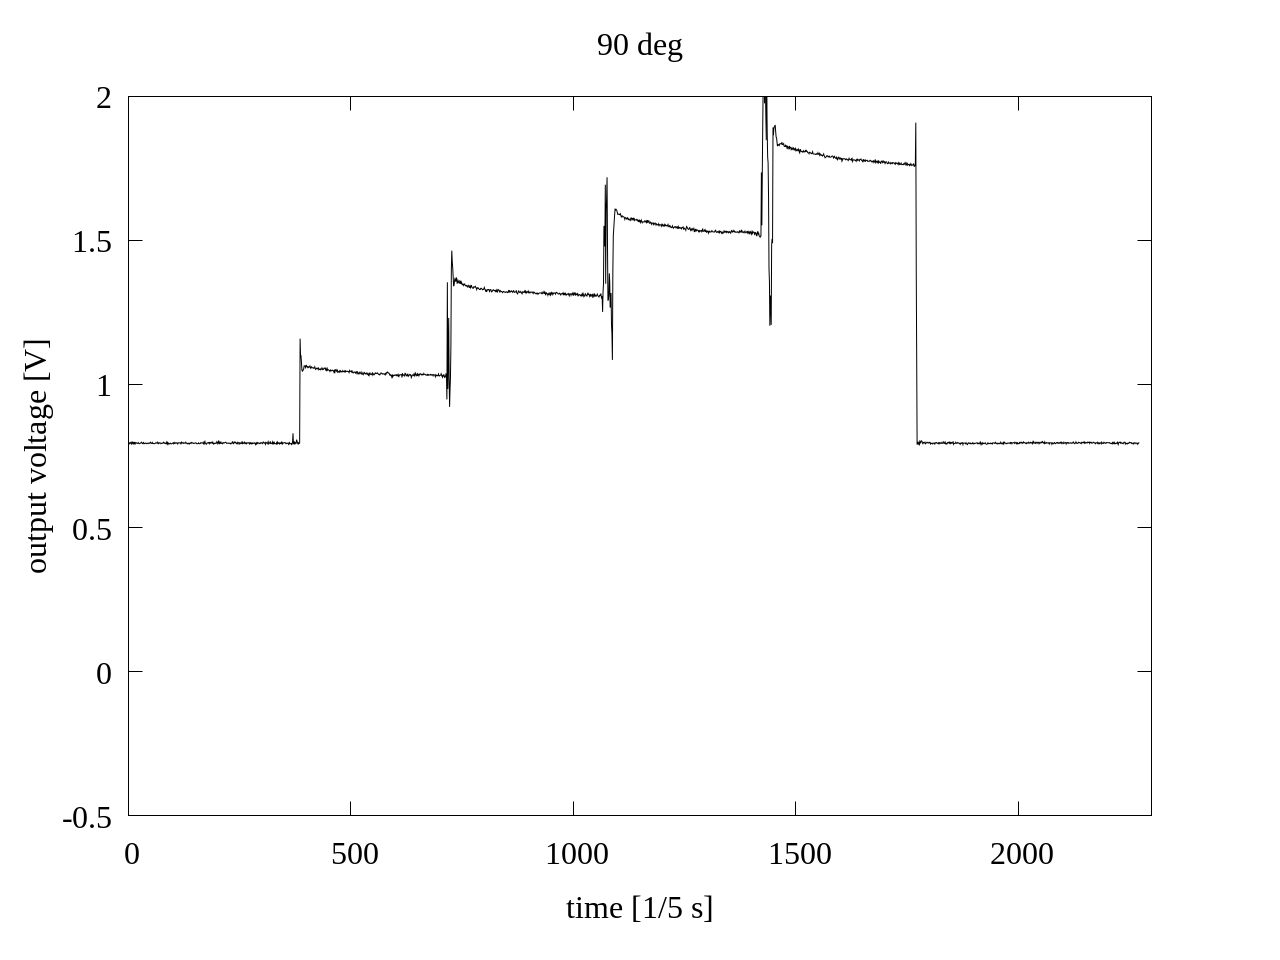
\includegraphics[width=88mm]{../images/reverse/90_loadcell.png}
        \caption{Result of loadcell voltage}
        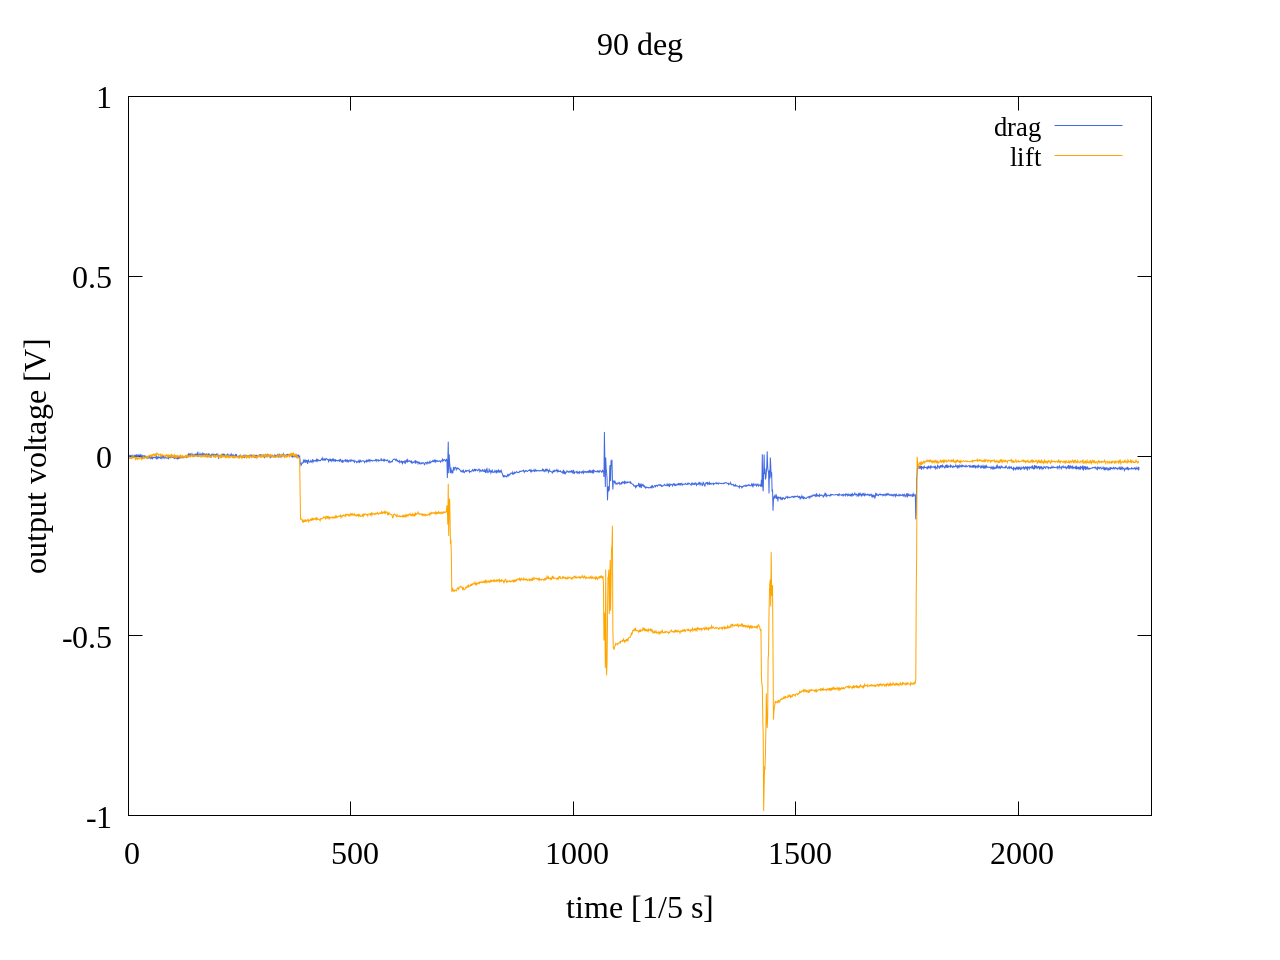
\includegraphics[width=88mm]{../images/reverse/90_strainsensor.png}
        \caption{Result of strainsensor voltage}
    \end{center}
\end{figure}

\newpage
\section{Drift correction}
\subsection{0 deg}
\begin{figure}[htbp]
    \footnotesize
    \begin{center}
        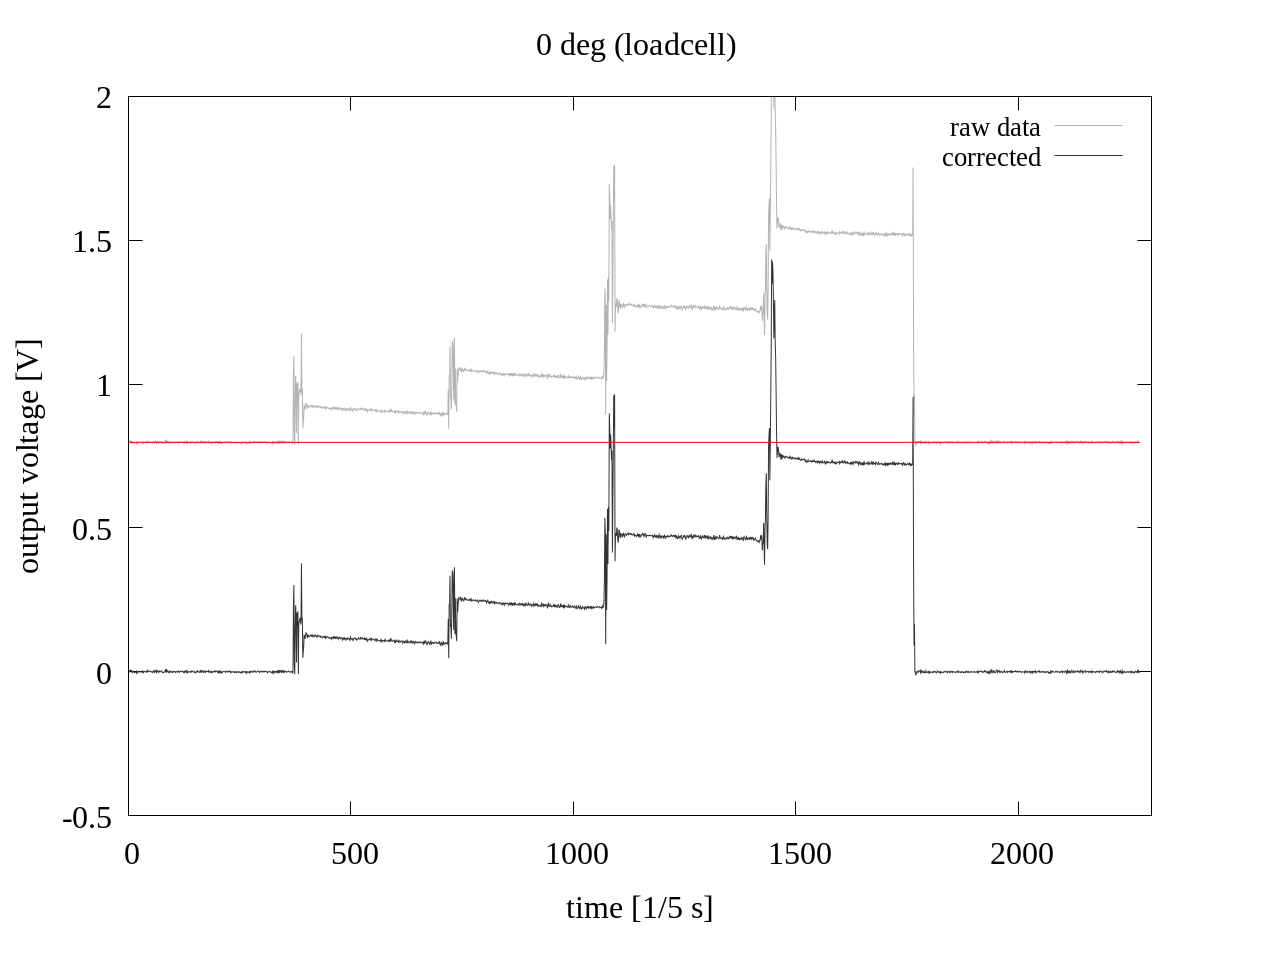
\includegraphics[width=88mm]{../images/drift/0_loadcell_drift.png}
        \caption{Drift correction (loadcell)}
        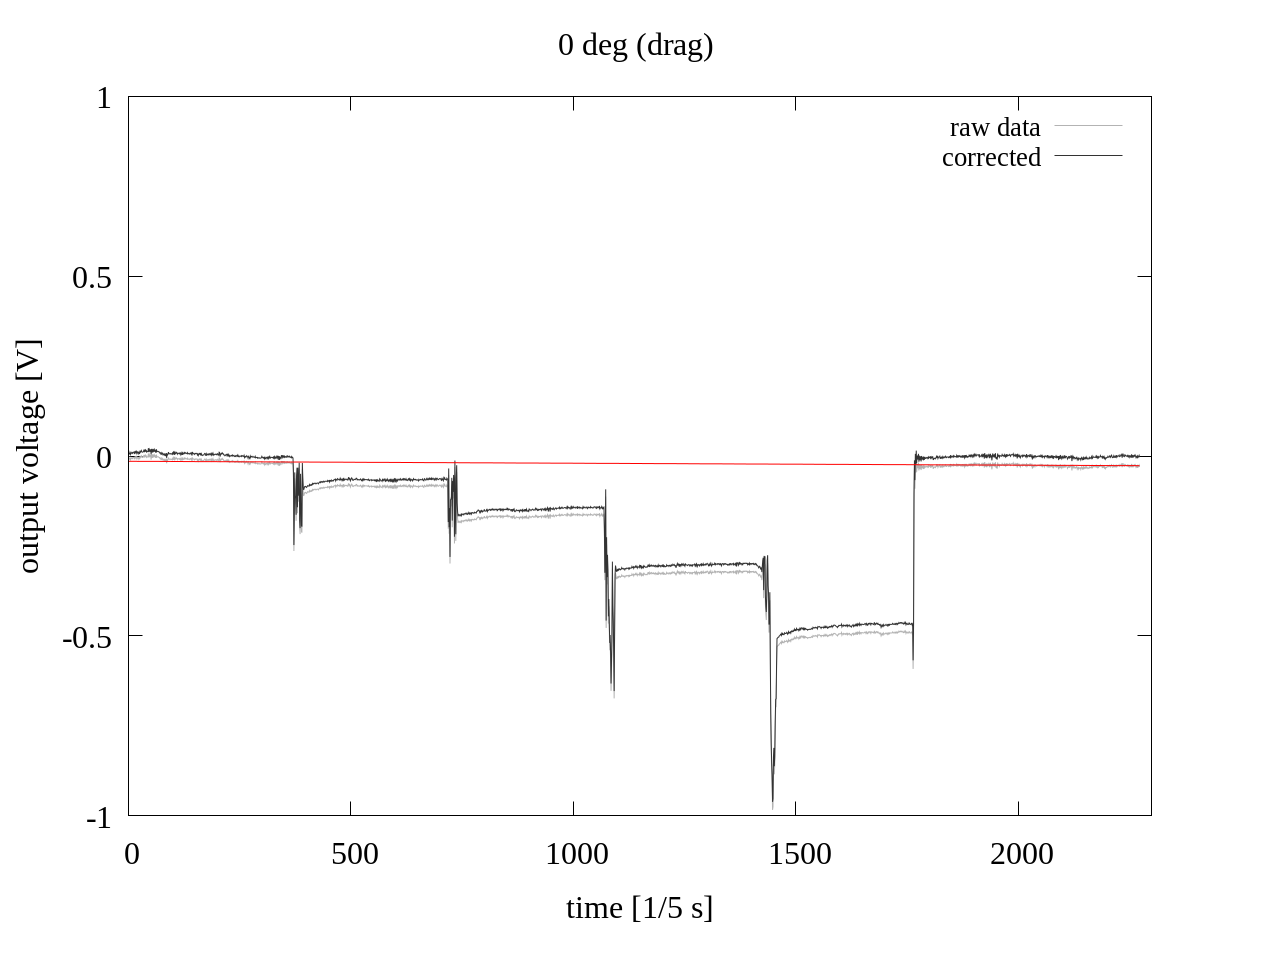
\includegraphics[width=88mm]{../images/drift/0_drag_drift.png}
        \caption{Drift correction (drag)}
        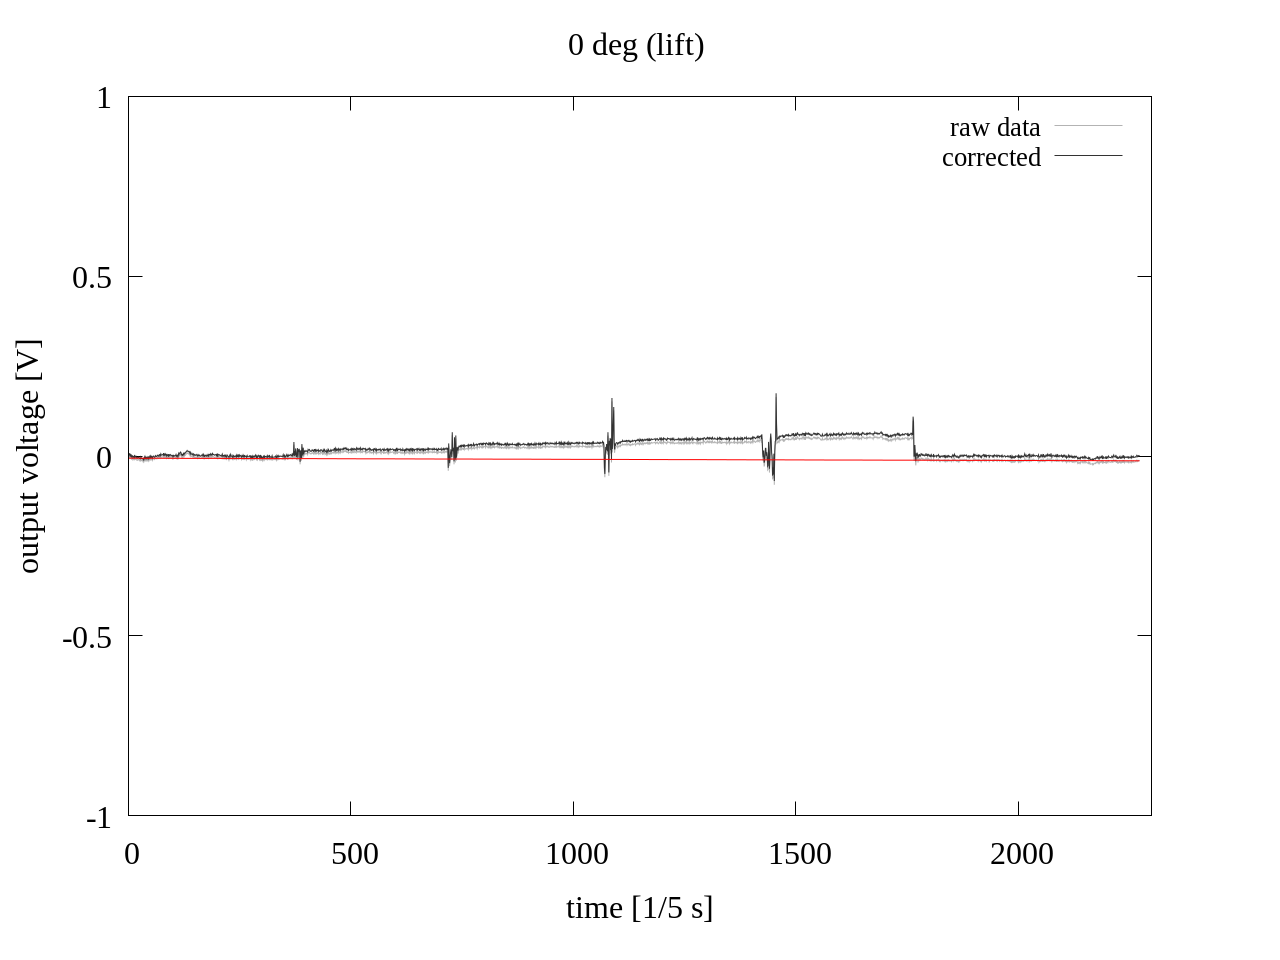
\includegraphics[width=88mm]{../images/drift/0_lift_drift.png}
        \caption{Drift correction (lift)}
    \end{center}
\end{figure}

\newpage
\subsection{30 deg}
\begin{figure}[htbp]
    \footnotesize
    \begin{center}
        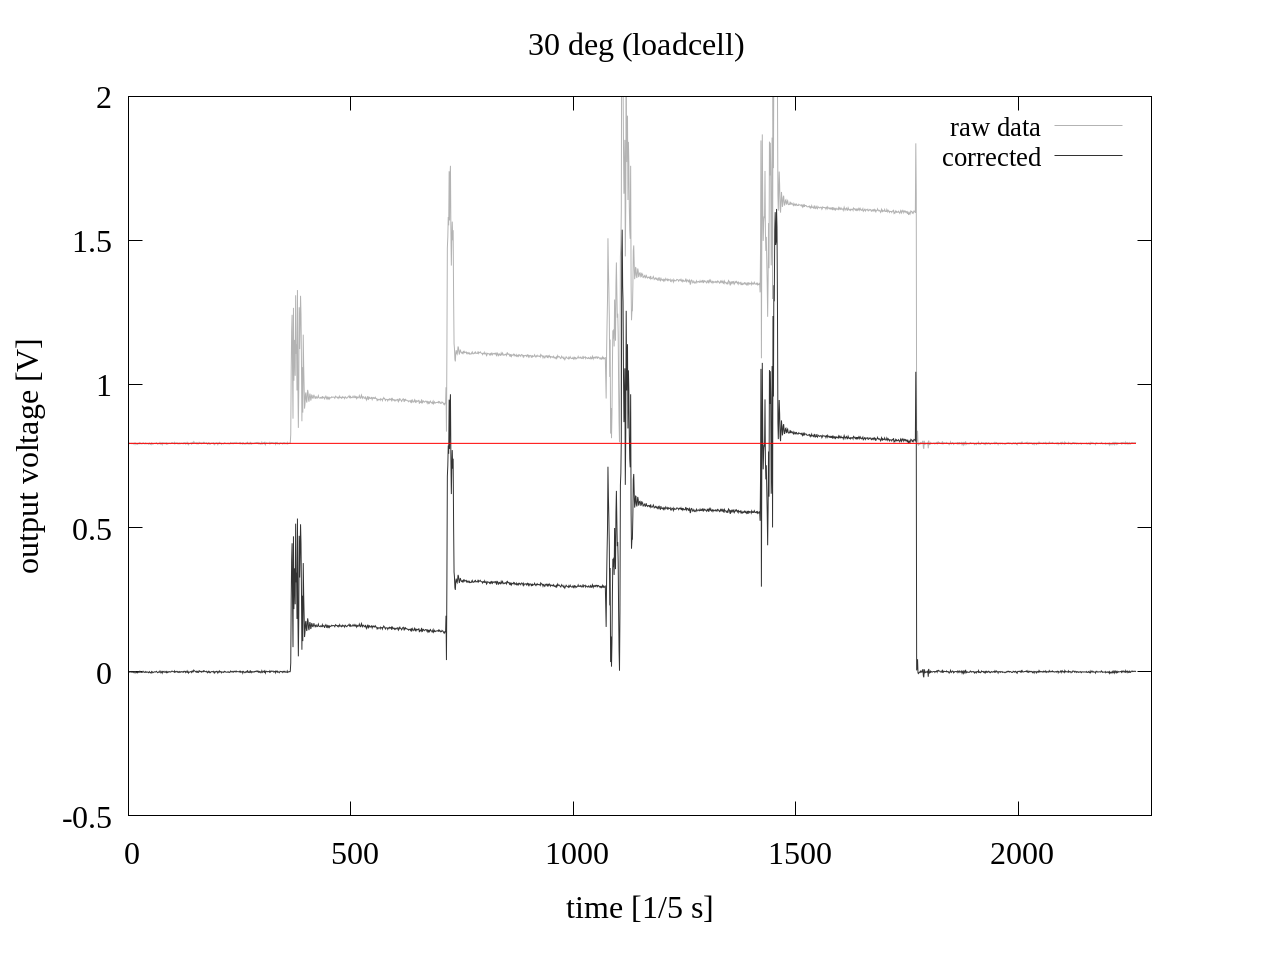
\includegraphics[width=88mm]{../images/drift/30_loadcell_drift.png}
        \caption{Drift correction (loadcell)}
        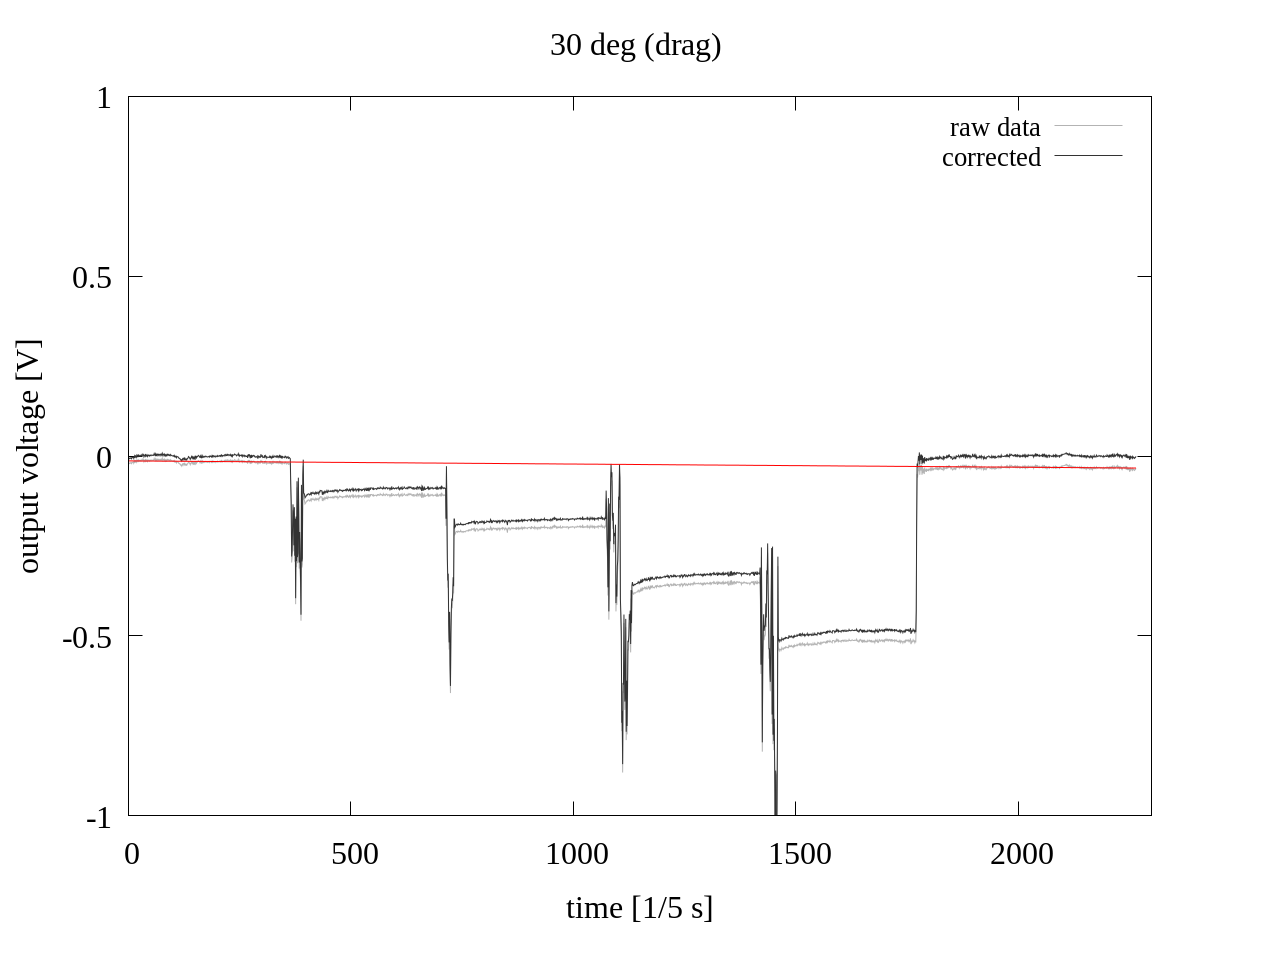
\includegraphics[width=88mm]{../images/drift/30_drag_drift.png}
        \caption{Drift correction (drag)}
        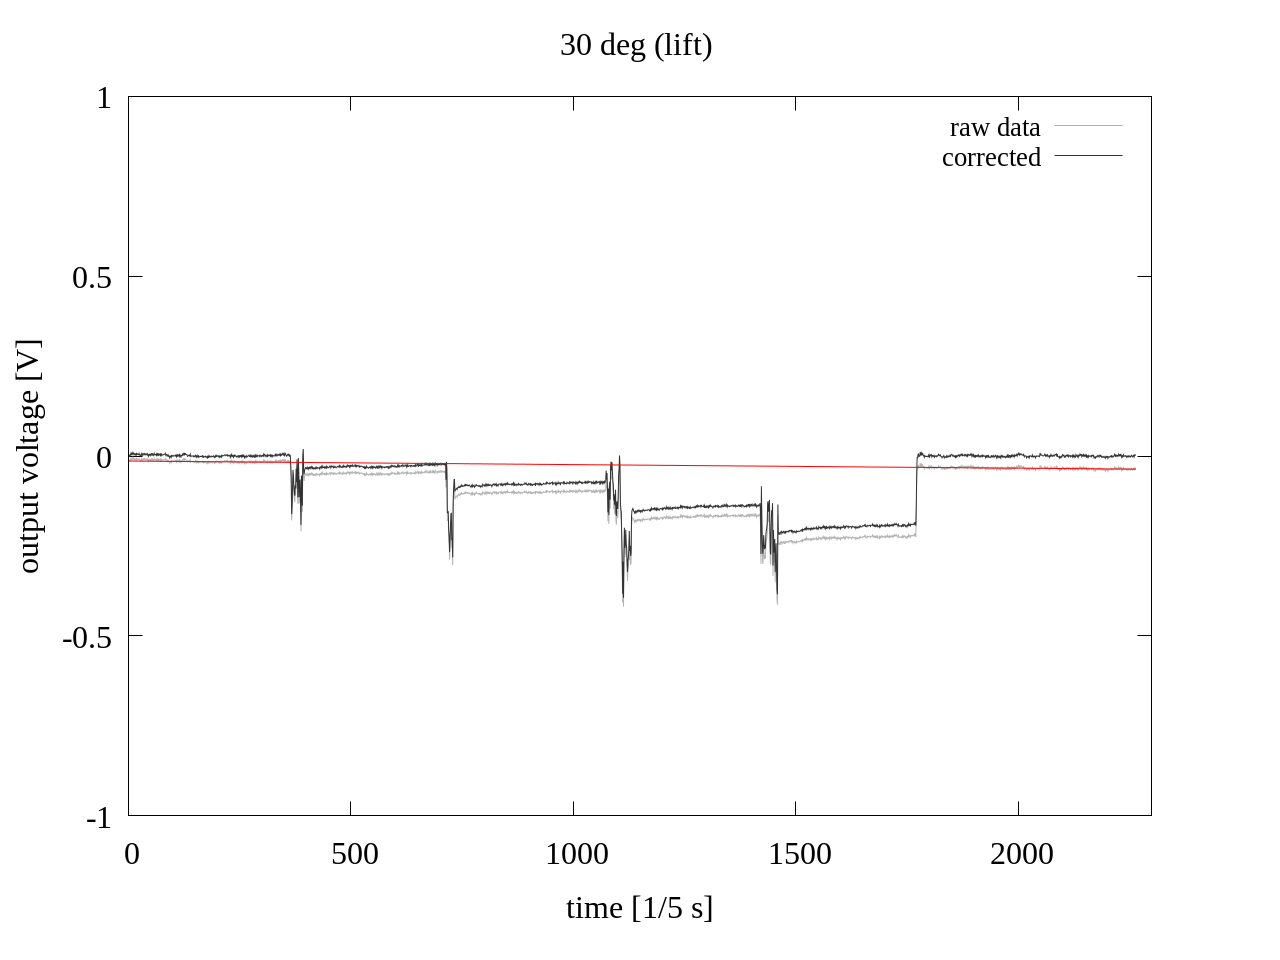
\includegraphics[width=88mm]{../images/drift/30_lift_drift.png}
        \caption{Drift correction (lift)}
    \end{center}
\end{figure}

\newpage
\subsection{45 deg}
\begin{figure}[htbp]
    \footnotesize
    \begin{center}
        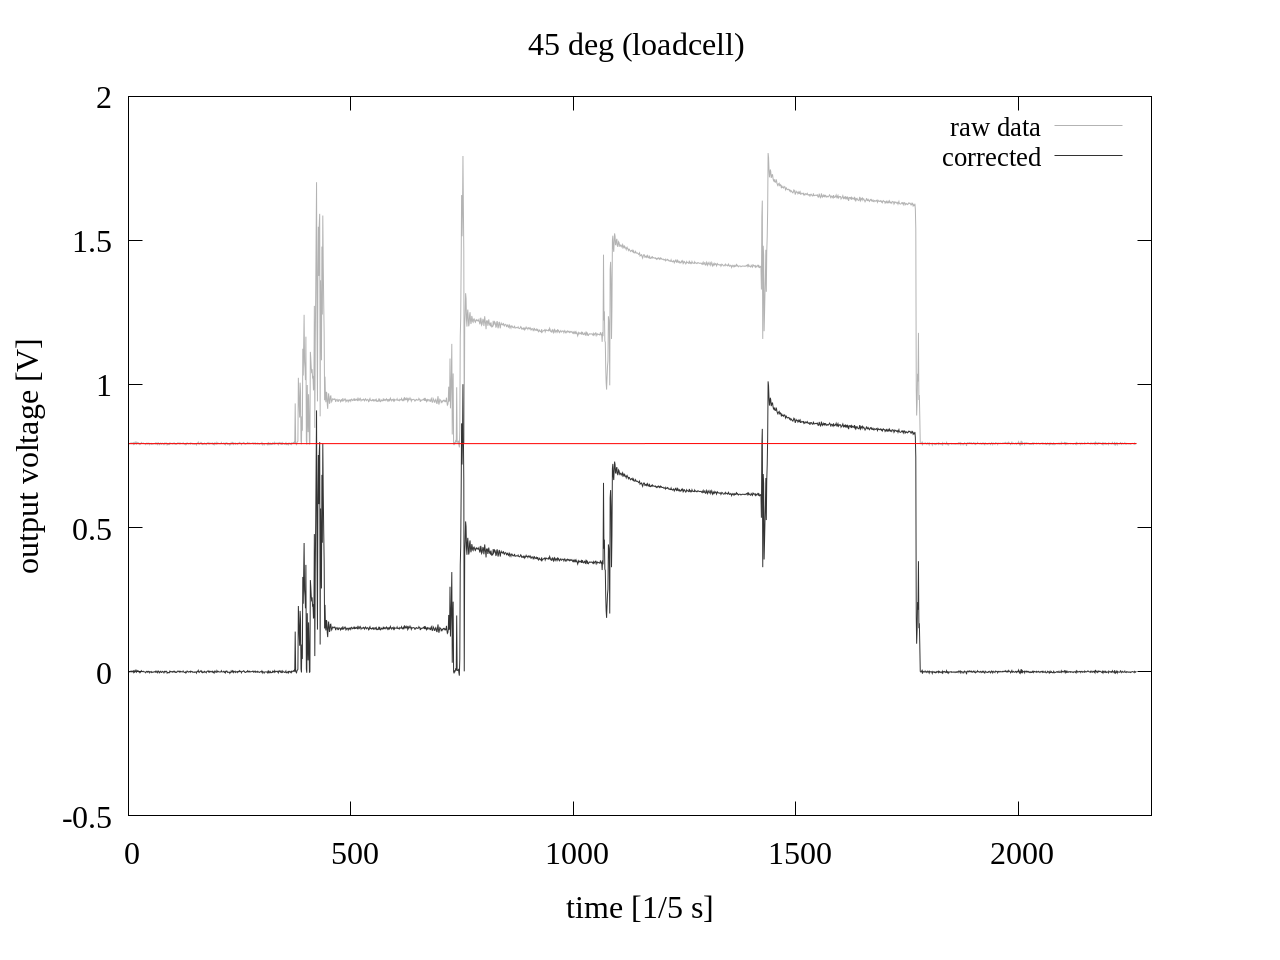
\includegraphics[width=88mm]{../images/drift/45_loadcell_drift.png}
        \caption{Drift correction (loadcell)}
        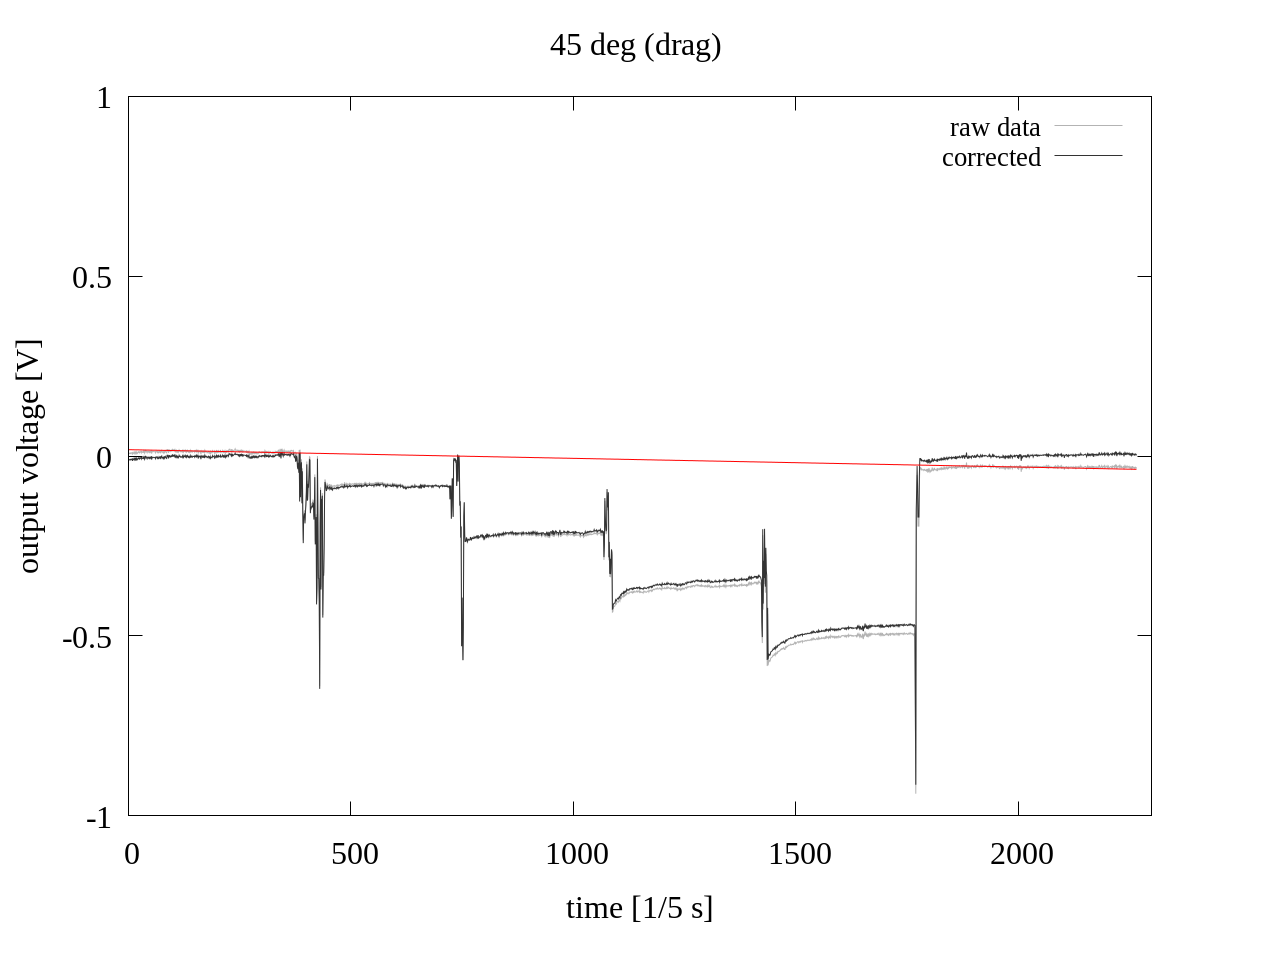
\includegraphics[width=88mm]{../images/drift/45_drag_drift.png}
        \caption{Drift correction (drag)}
        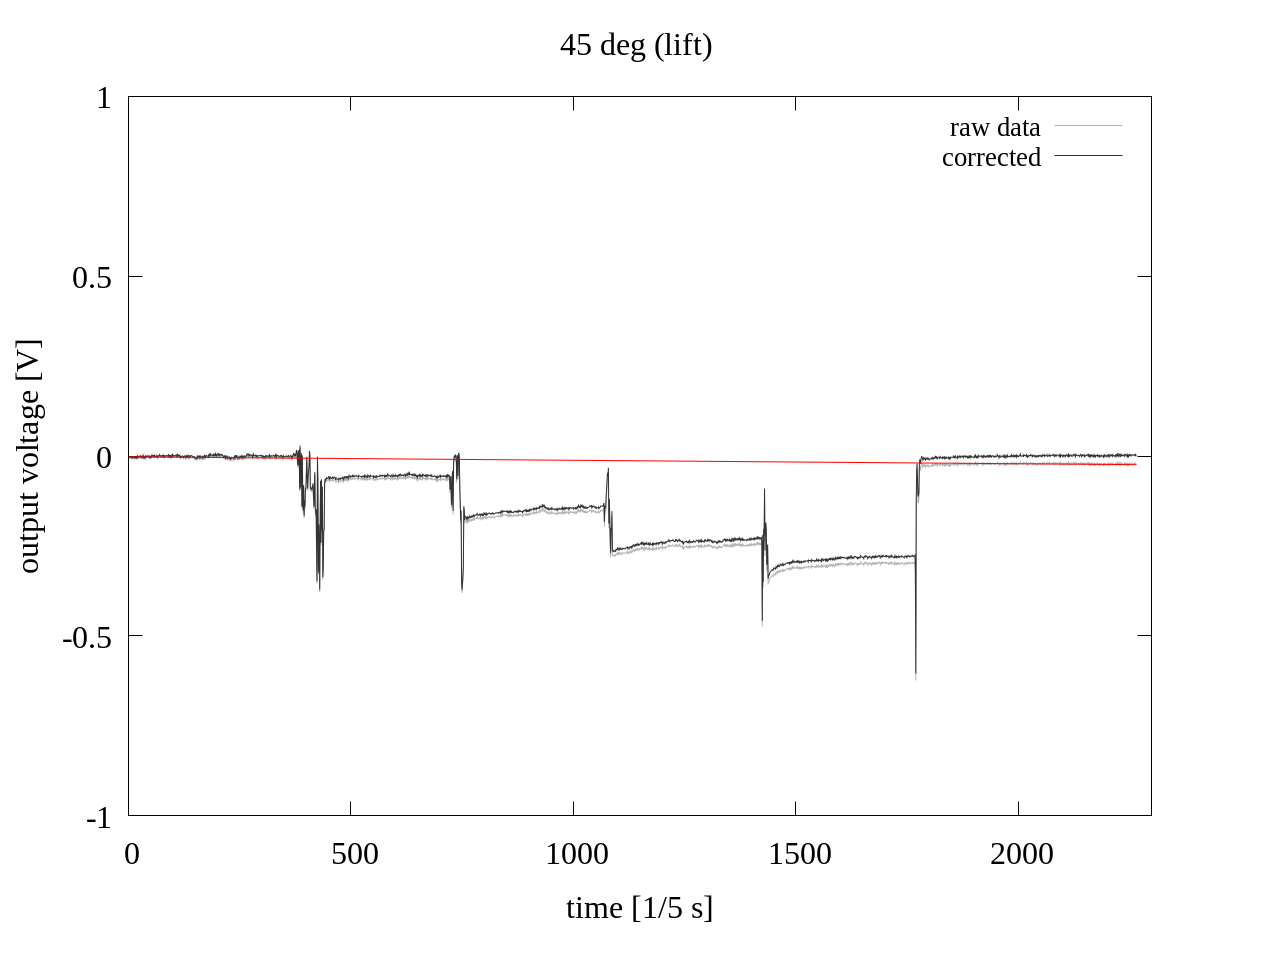
\includegraphics[width=88mm]{../images/drift/45_lift_drift.png}
        \caption{Drift correction (lift)}
    \end{center}
\end{figure}

\newpage
\subsection{60 deg}
\begin{figure}[htbp]
    \footnotesize
    \begin{center}
        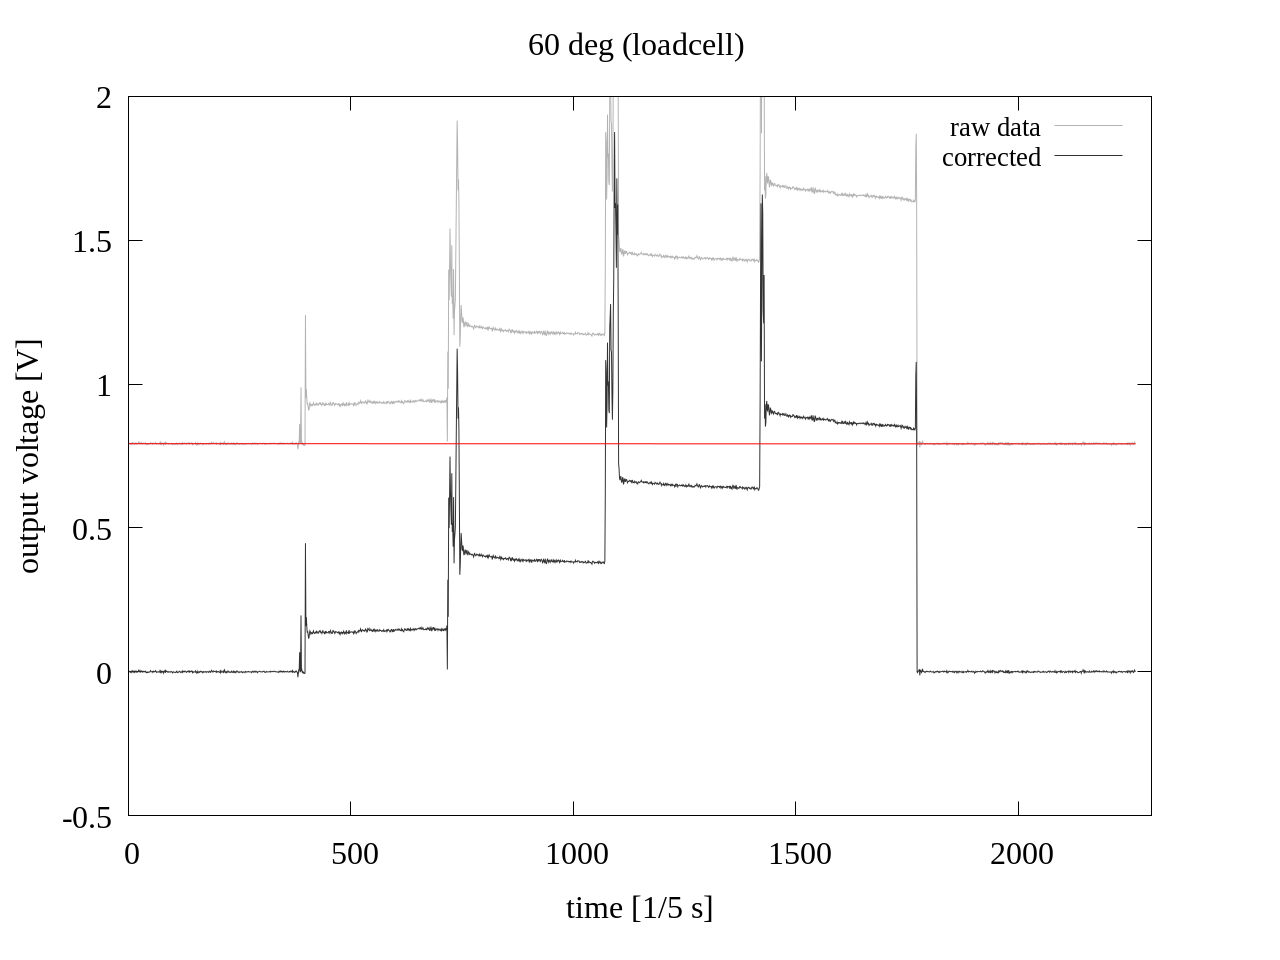
\includegraphics[width=88mm]{../images/drift/60_loadcell_drift.png}
        \caption{Drift correction (loadcell)}
        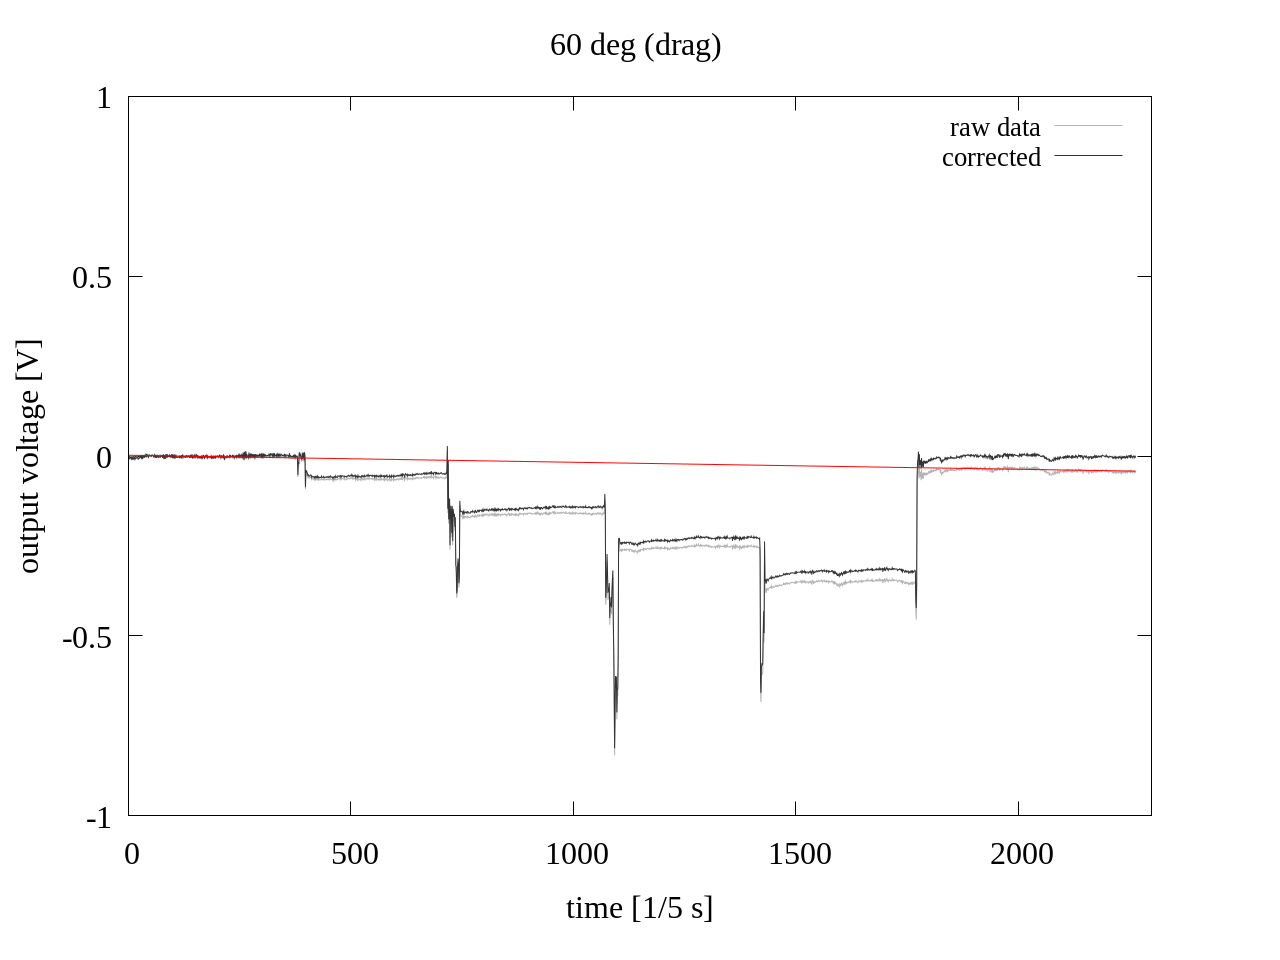
\includegraphics[width=88mm]{../images/drift/60_drag_drift.png}
        \caption{Drift correction (drag)}
        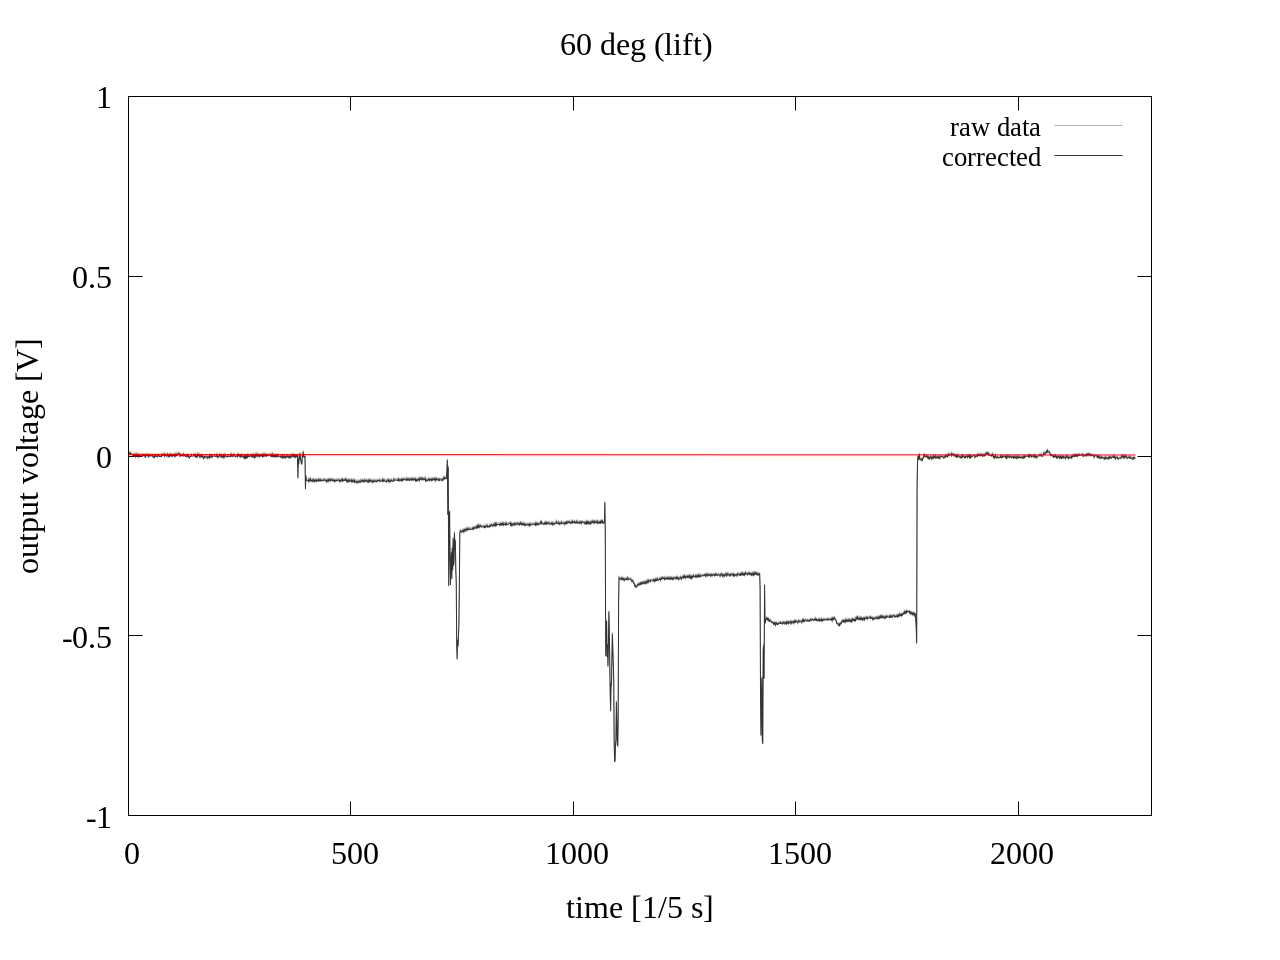
\includegraphics[width=88mm]{../images/drift/60_lift_drift.png}
        \caption{Drift correction (lift)}
    \end{center}
\end{figure}

\newpage
\subsection{75 deg}
\begin{figure}[htbp]
    \footnotesize
    \begin{center}
        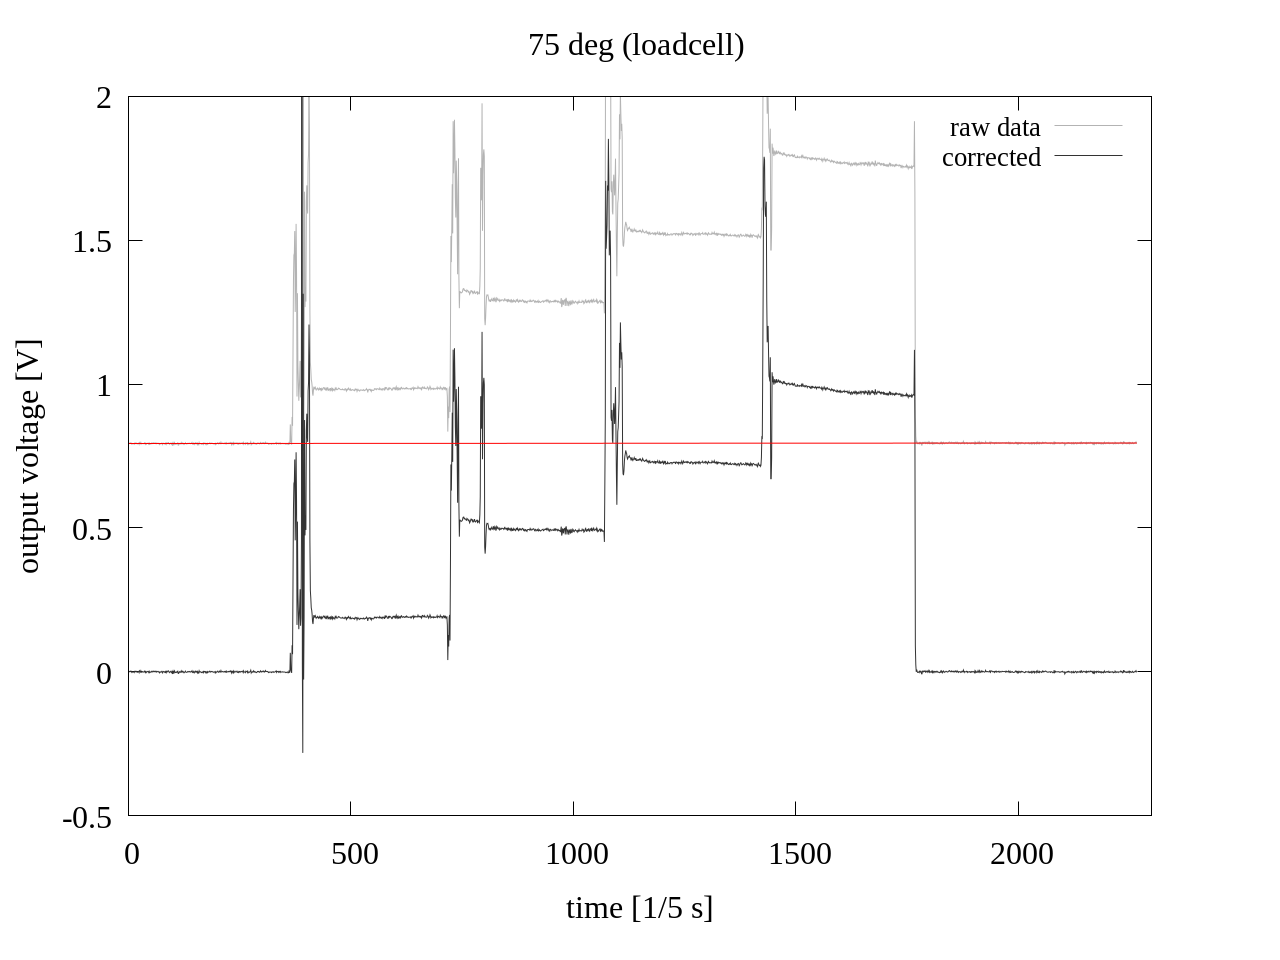
\includegraphics[width=88mm]{../images/drift/75_loadcell_drift.png}
        \caption{Drift correction (loadcell)}
        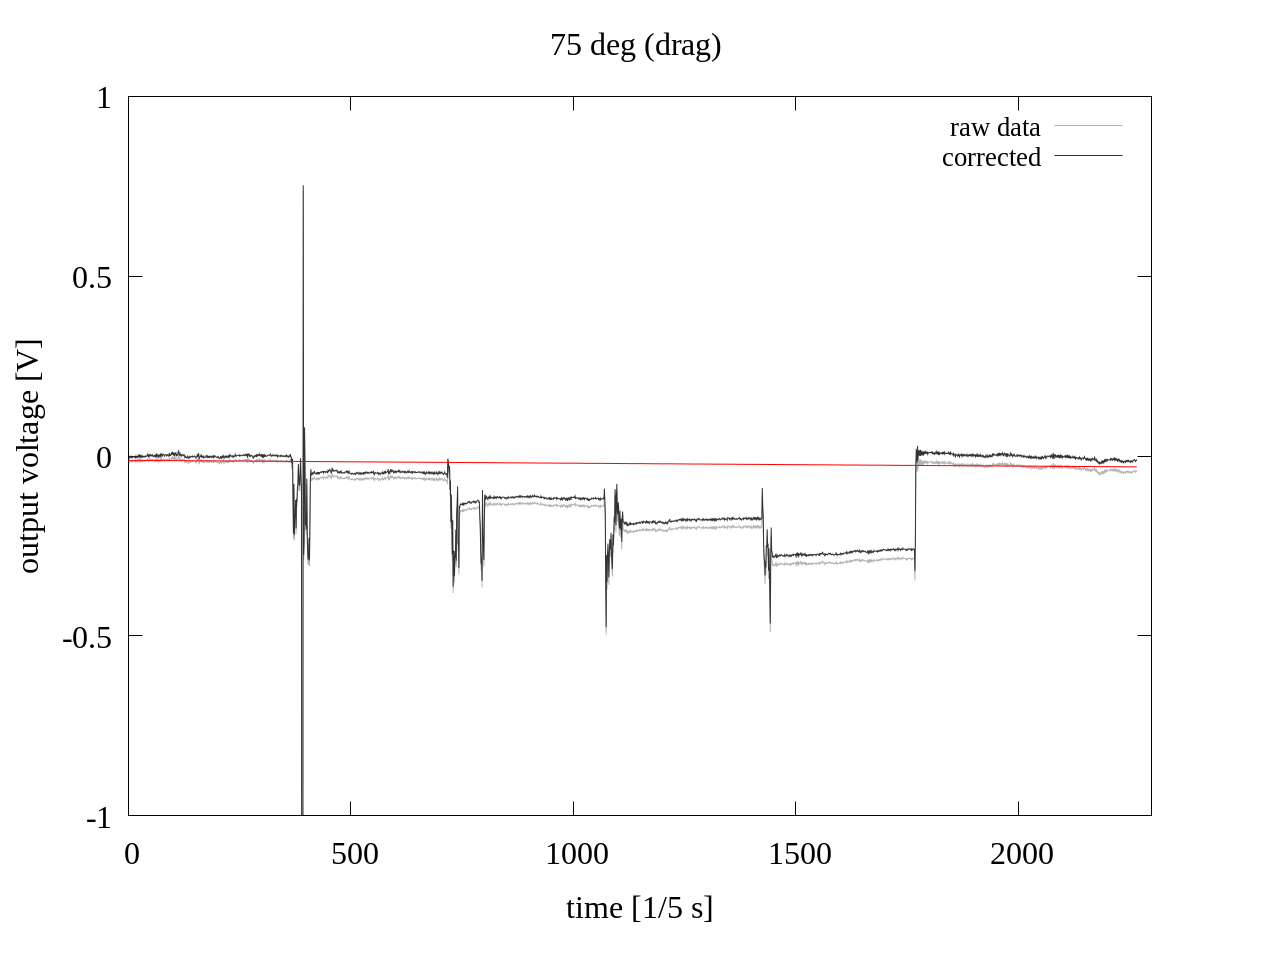
\includegraphics[width=88mm]{../images/drift/75_drag_drift.png}
        \caption{Drift correction (drag)}
        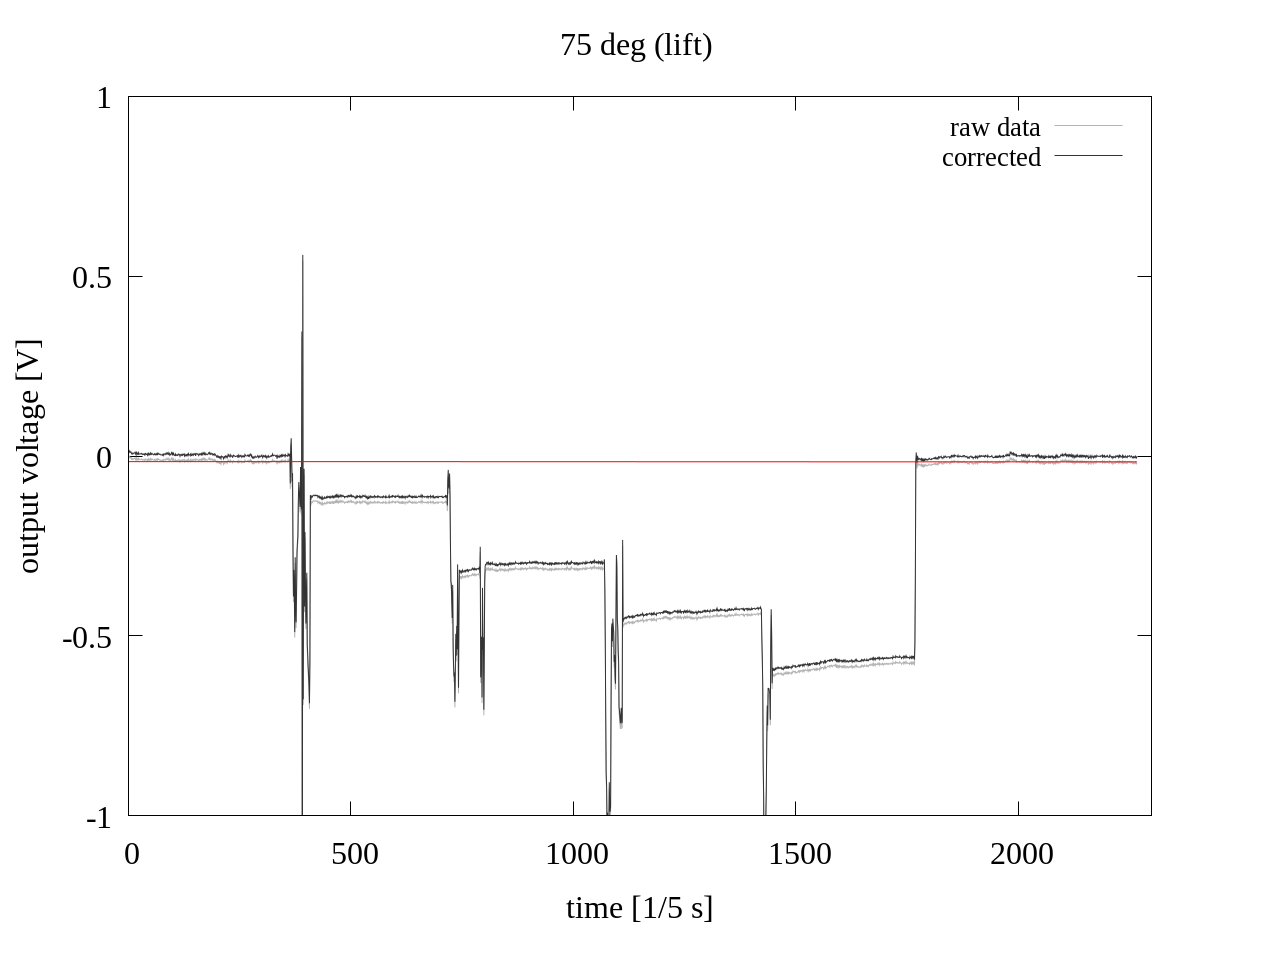
\includegraphics[width=88mm]{../images/drift/75_lift_drift.png}
        \caption{Drift correction (lift)}
    \end{center}
\end{figure}

\newpage
\subsection{90 deg}
\begin{figure}[htbp]
    \footnotesize
    \begin{center}
        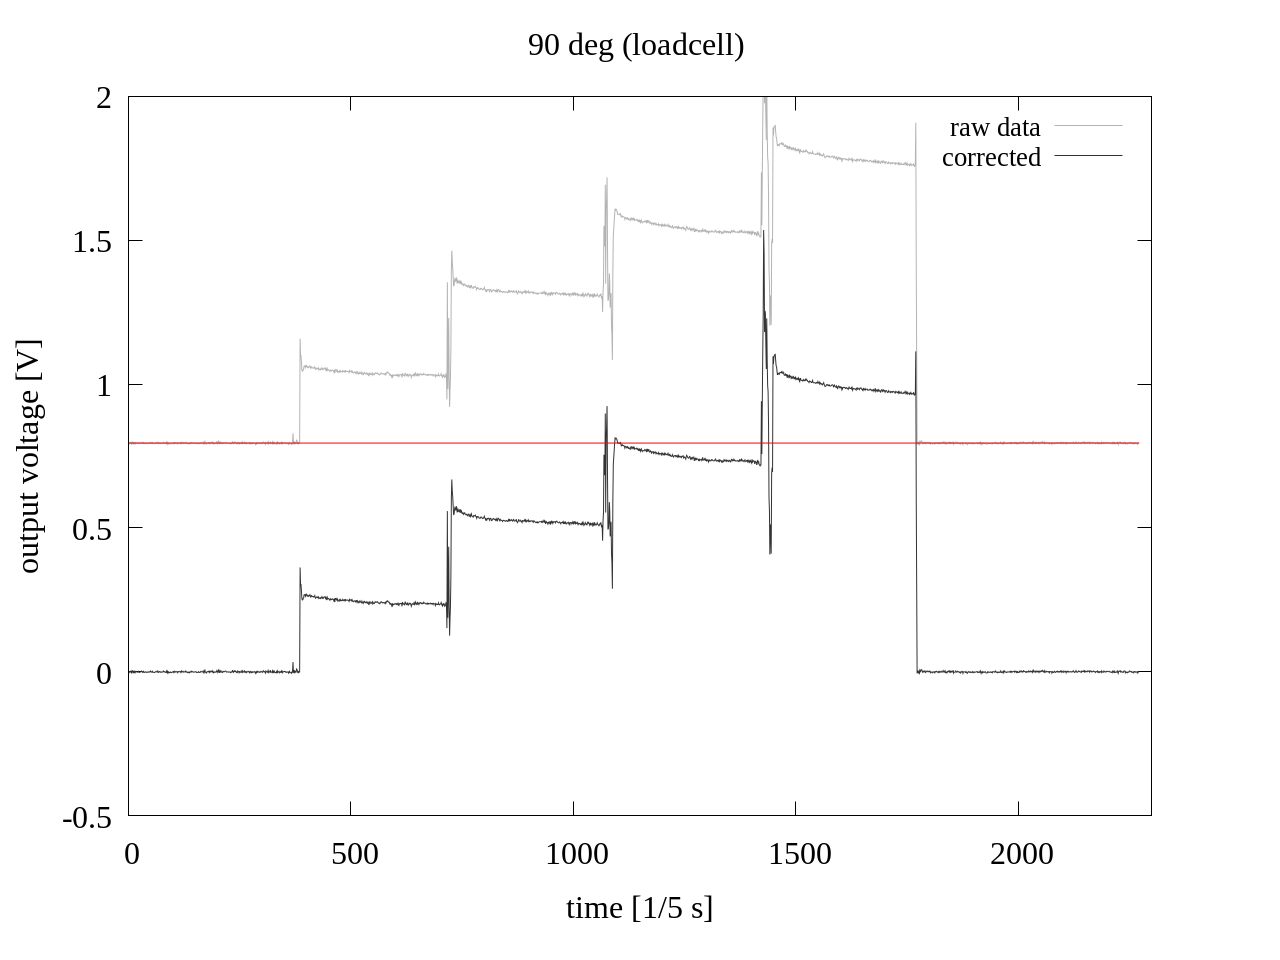
\includegraphics[width=88mm]{../images/drift/90_loadcell_drift.png}
        \caption{Drift correction (loadcell)}
        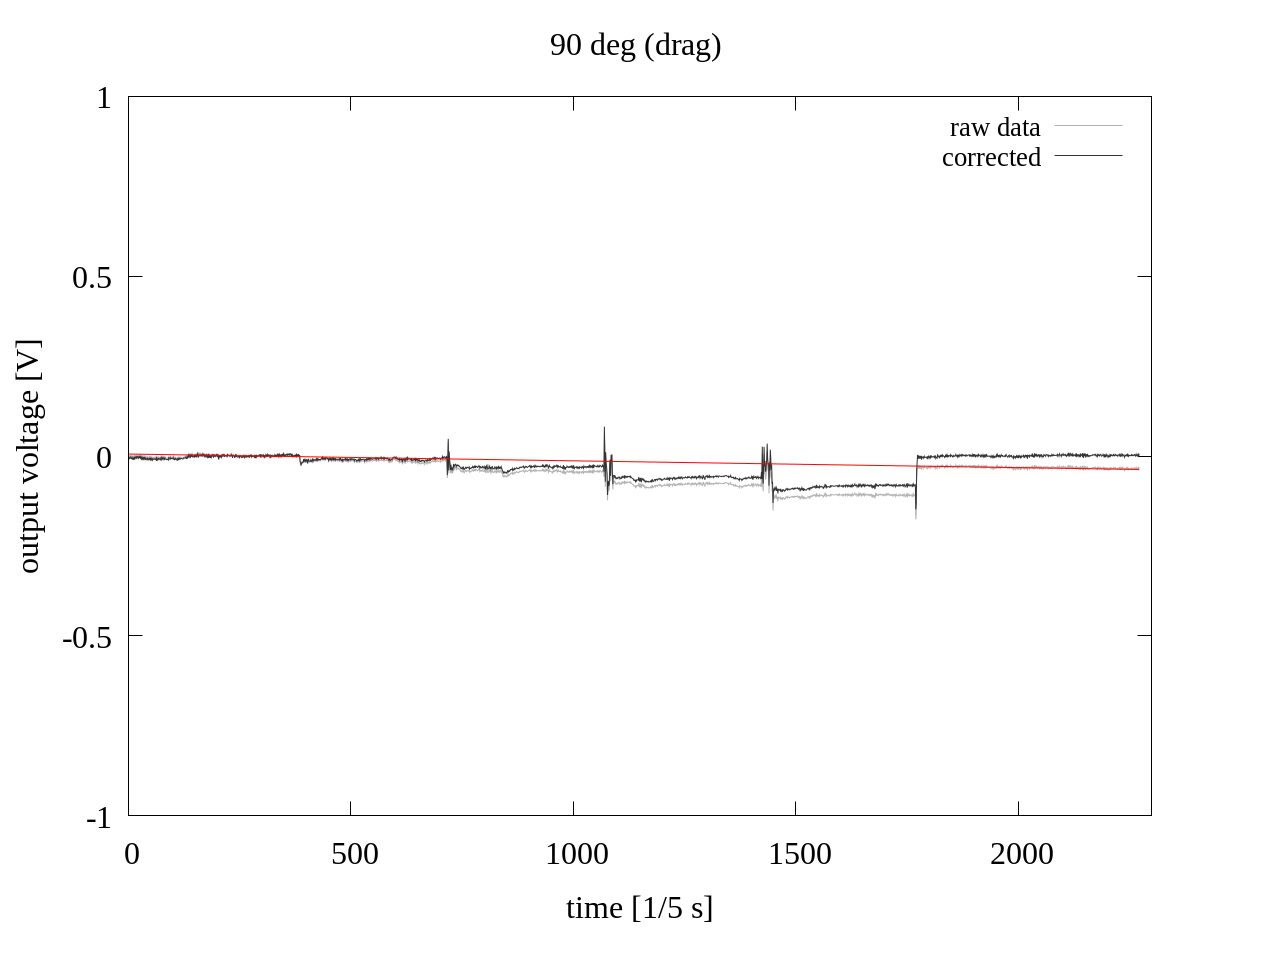
\includegraphics[width=88mm]{../images/drift/90_drag_drift.png}
        \caption{Drift correction (drag)}
        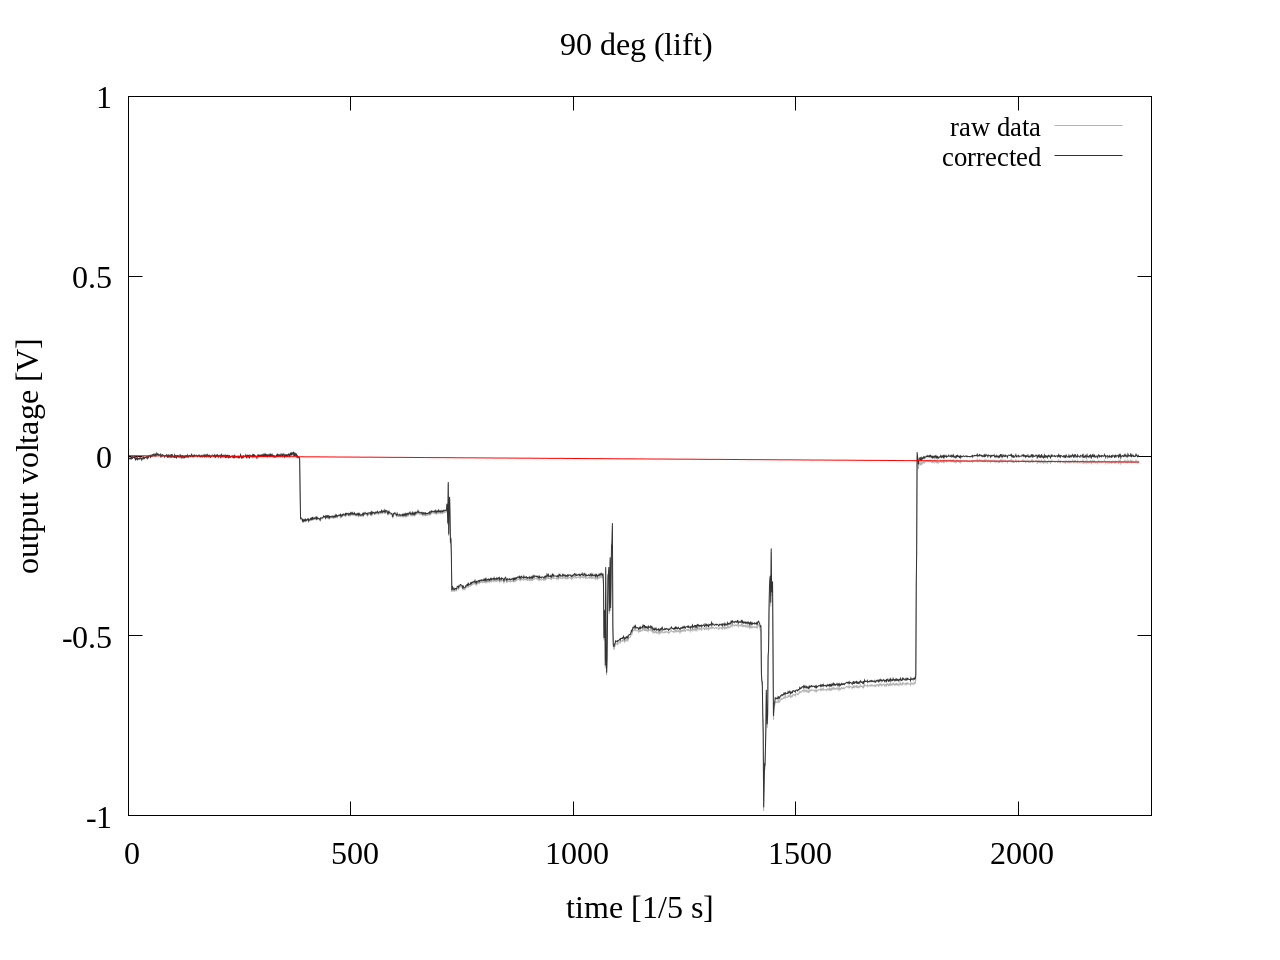
\includegraphics[width=88mm]{../images/drift/90_lift_drift.png}
        \caption{Drift correction (lift)}
    \end{center}
\end{figure}

\newpage
\section{Average}
\subsection{0 deg}
\begin{figure}[htbp]
    \footnotesize
    \begin{center}
        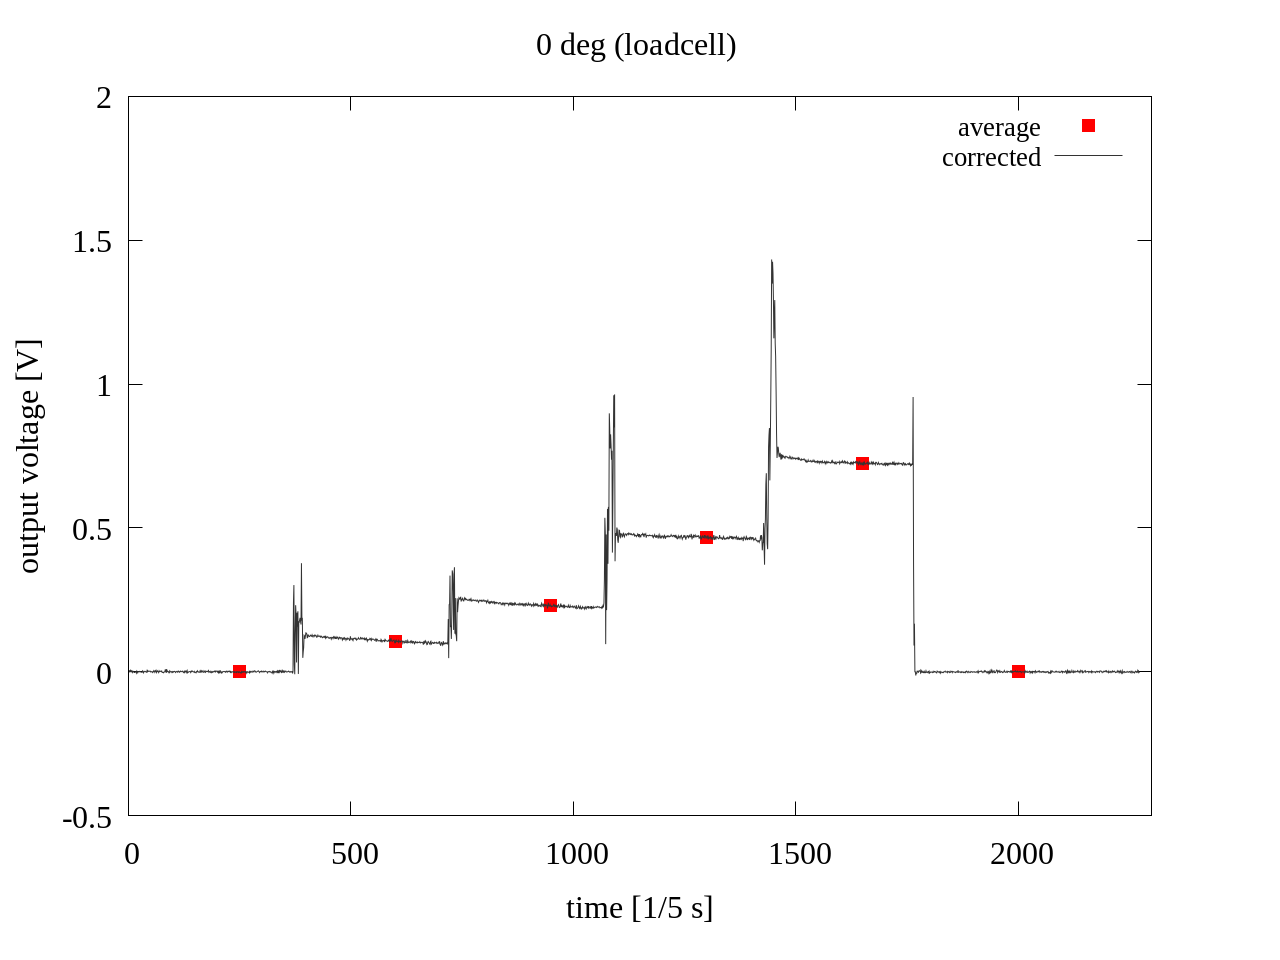
\includegraphics[width=88mm]{../images/average/0_loadcell_average.png}
        \caption{Average (loadcell)}
        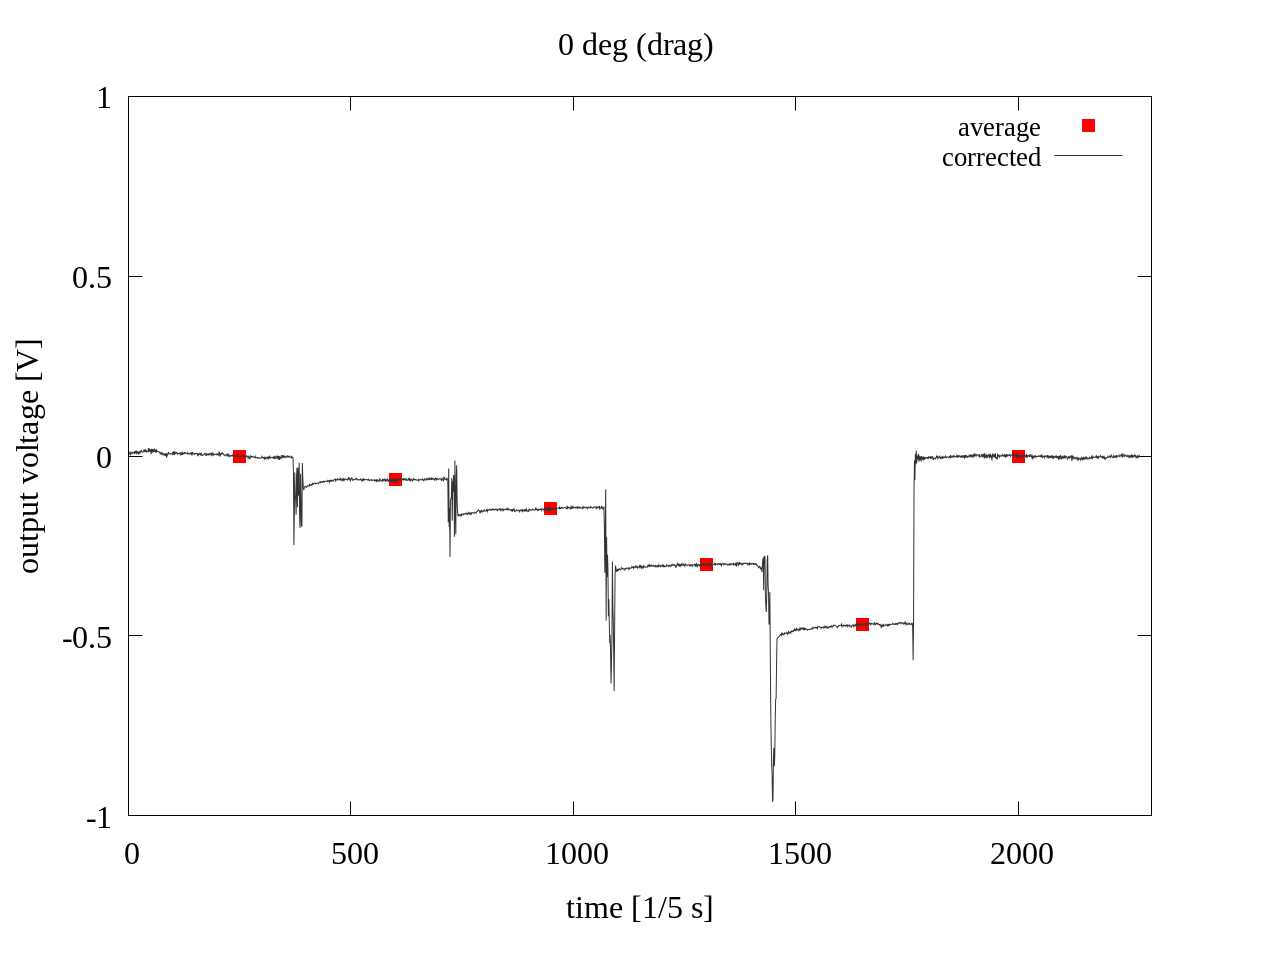
\includegraphics[width=88mm]{../images/average/0_drag_average.png}
        \caption{Average (drag)}
        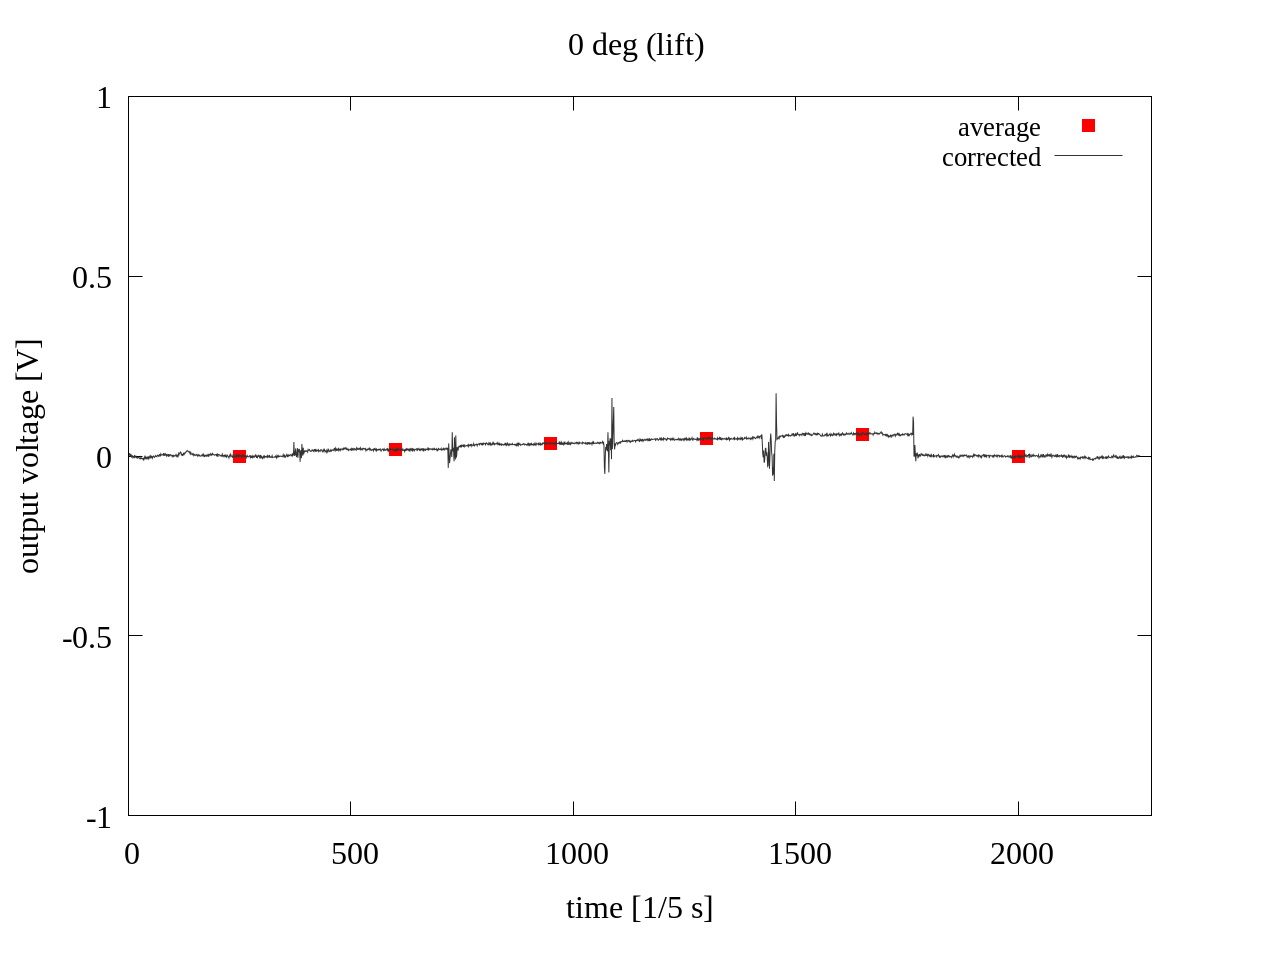
\includegraphics[width=88mm]{../images/average/0_lift_average.png}
        \caption{Average (lift)}
    \end{center}
\end{figure}

\newpage
\subsection{30 deg}
\begin{figure}[htbp]
    \footnotesize
    \begin{center}
        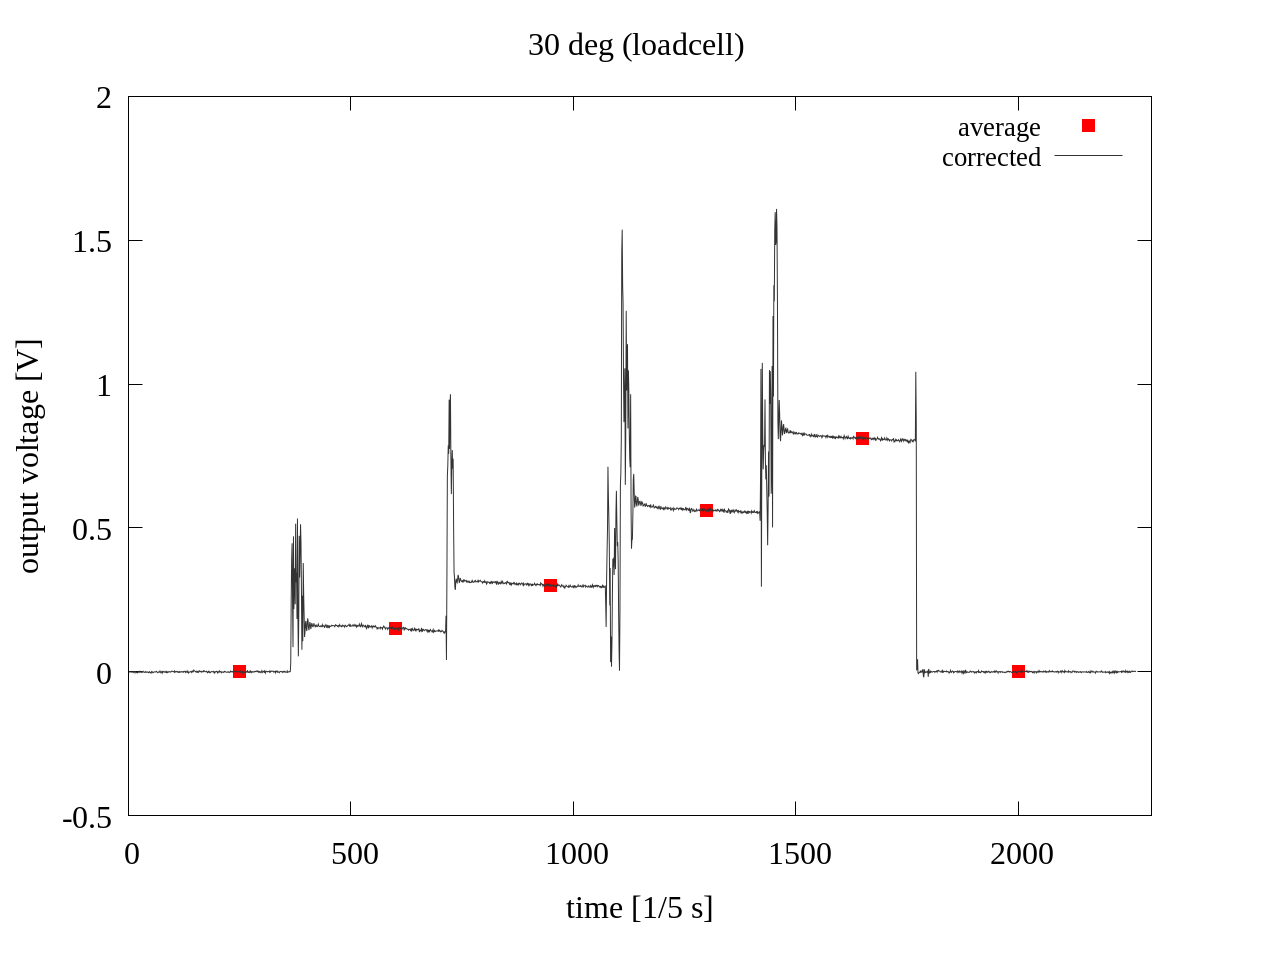
\includegraphics[width=88mm]{../images/average/30_loadcell_average.png}
        \caption{Average (loadcell)}
        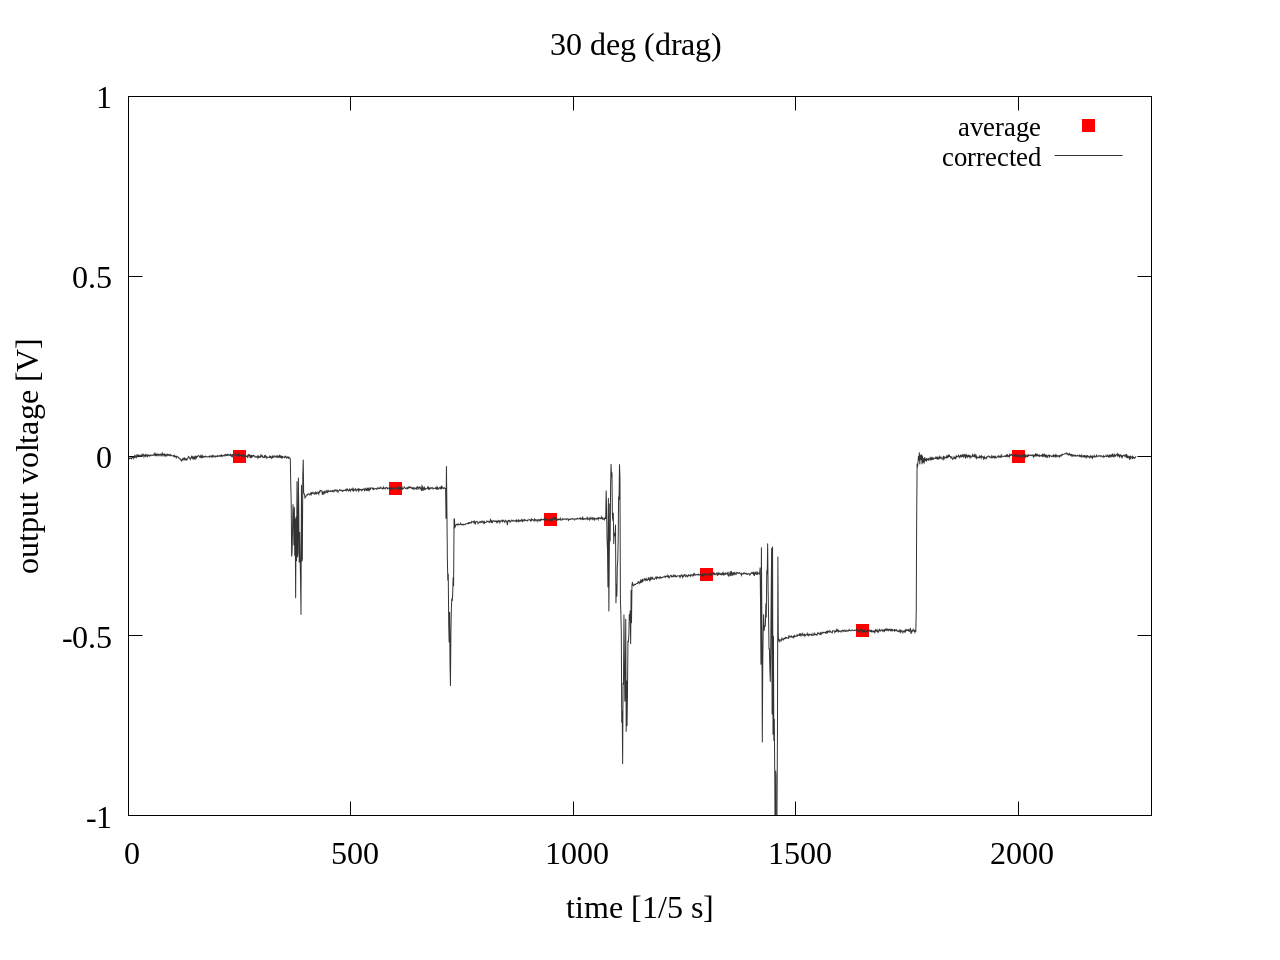
\includegraphics[width=88mm]{../images/average/30_drag_average.png}
        \caption{Average (drag)}
        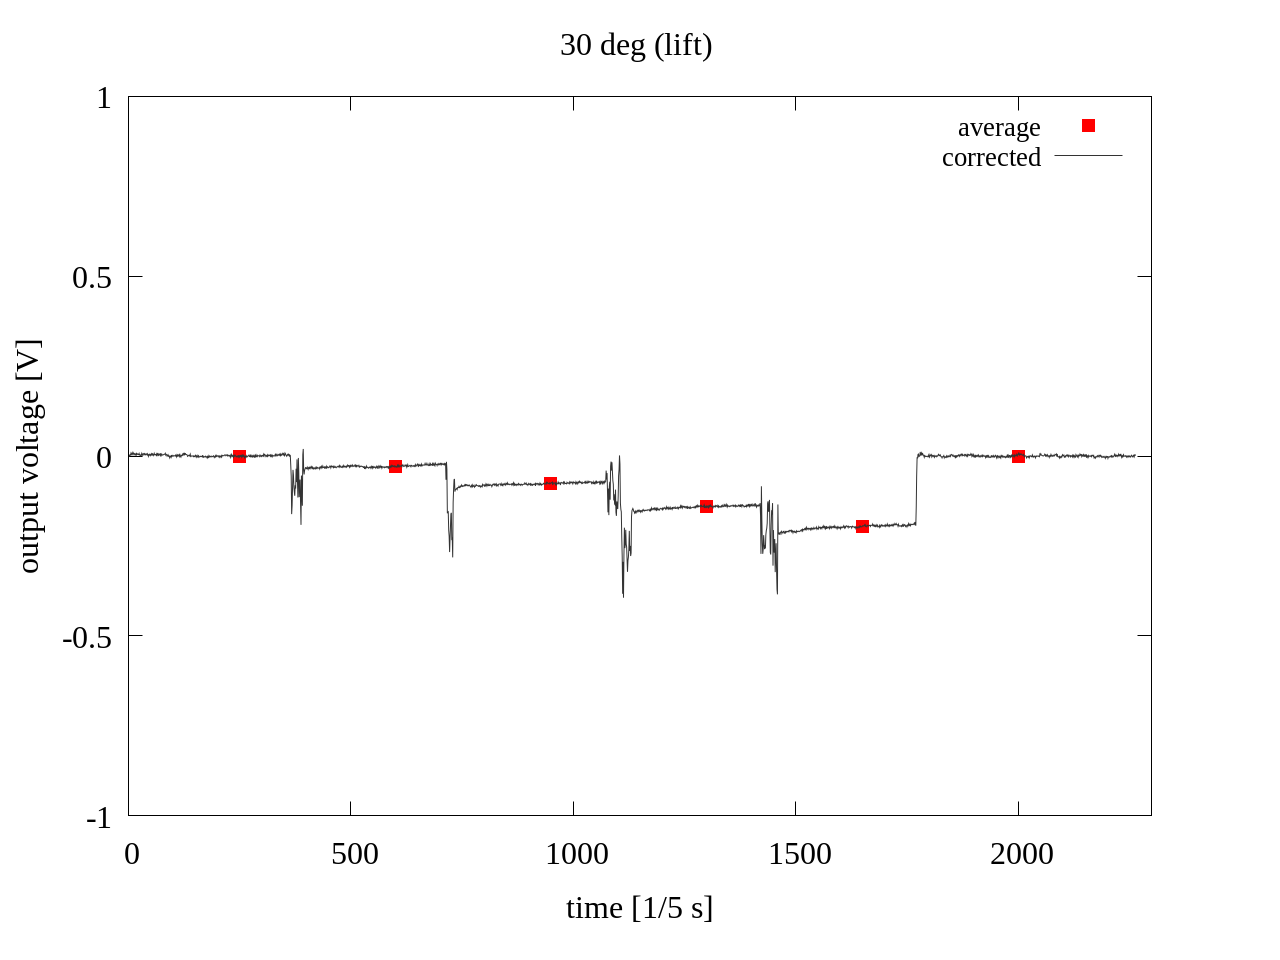
\includegraphics[width=88mm]{../images/average/30_lift_average.png}
        \caption{Average (lift)}
    \end{center}
\end{figure}

\newpage
\subsection{45 deg}
\begin{figure}[htbp]
    \footnotesize
    \begin{center}
        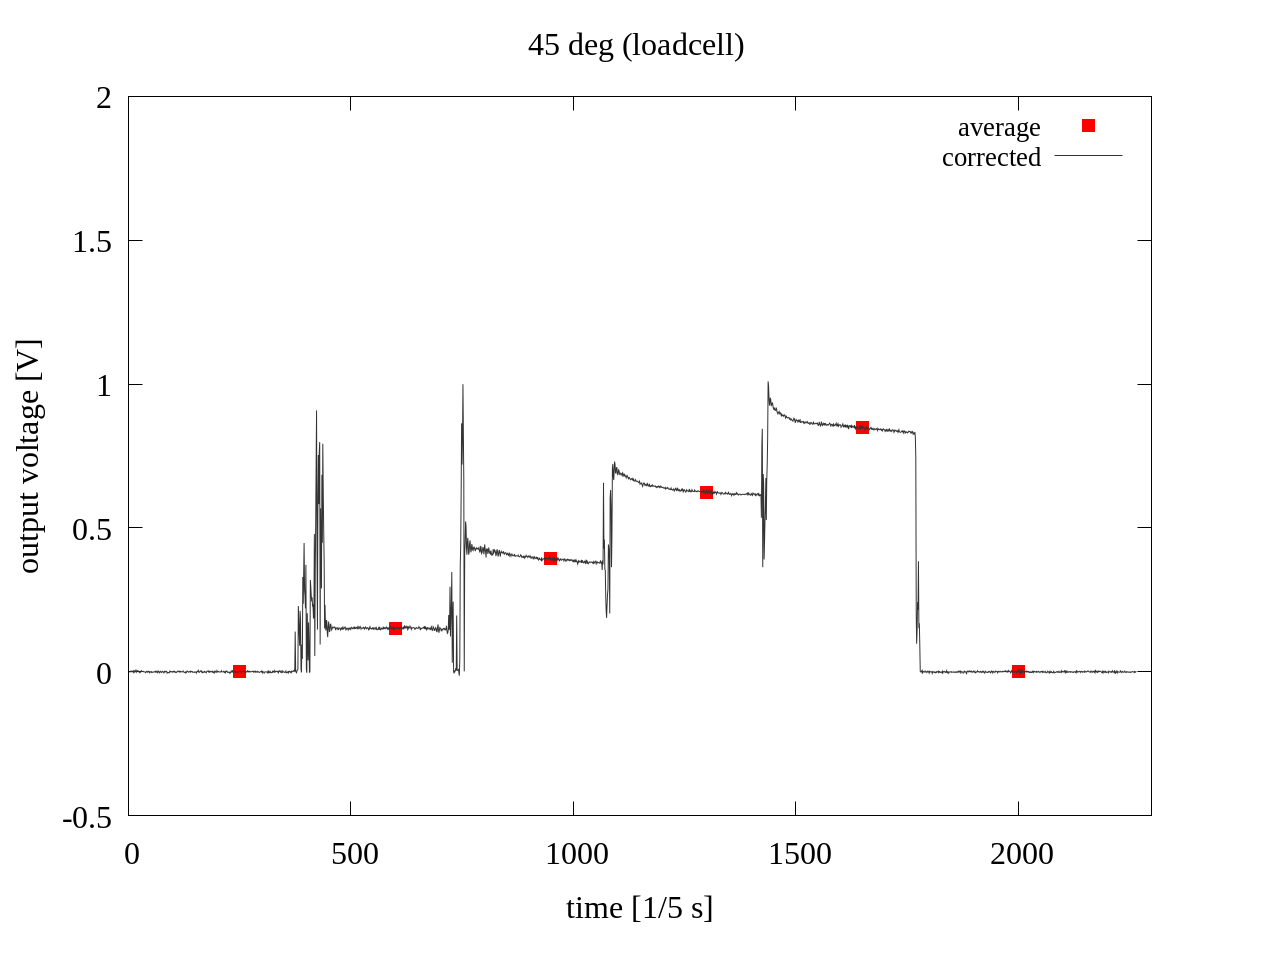
\includegraphics[width=88mm]{../images/average/45_loadcell_average.png}
        \caption{Average (loadcell)}
        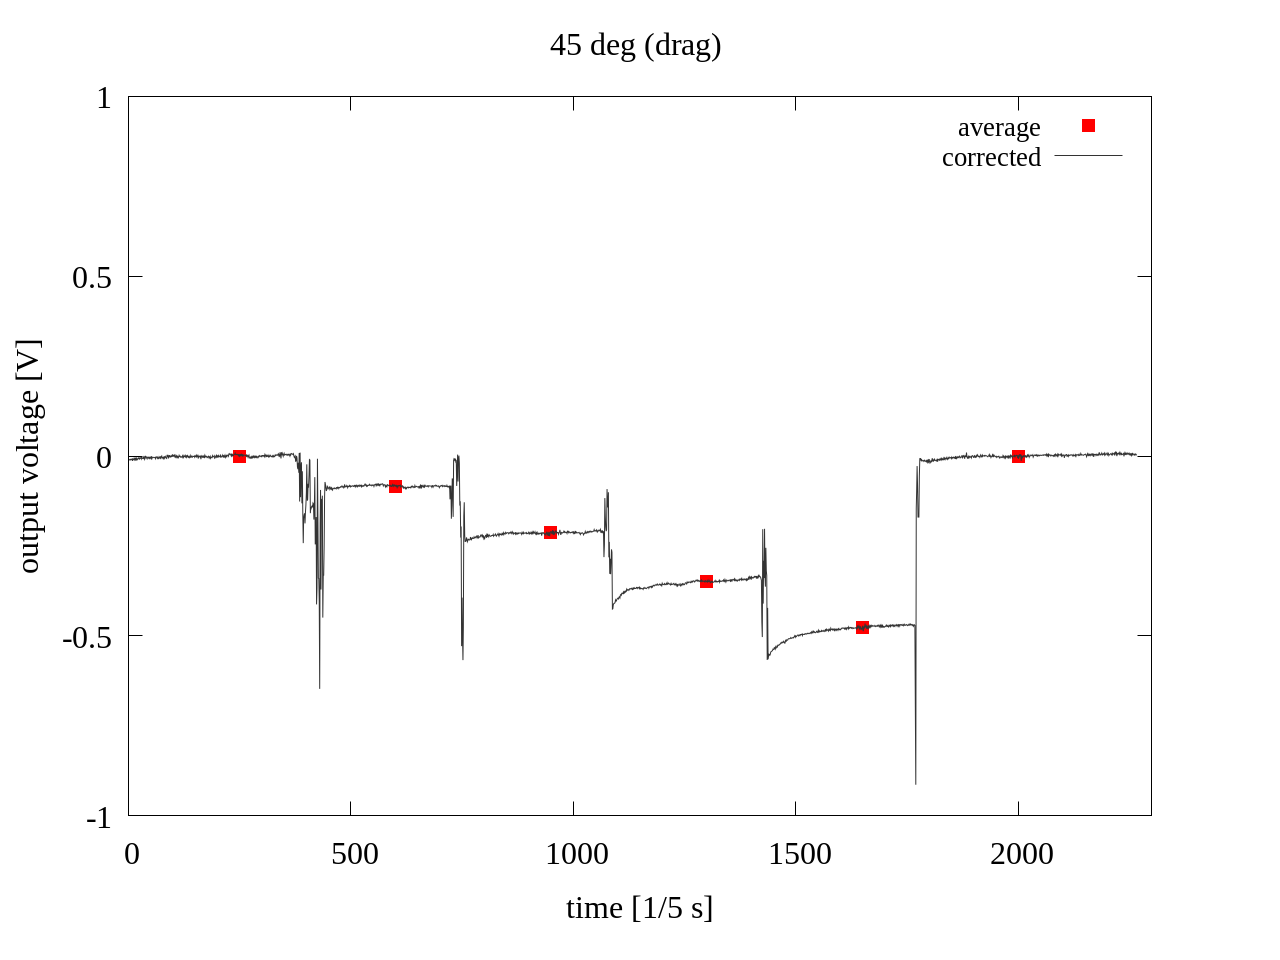
\includegraphics[width=88mm]{../images/average/45_drag_average.png}
        \caption{Average (drag)}
        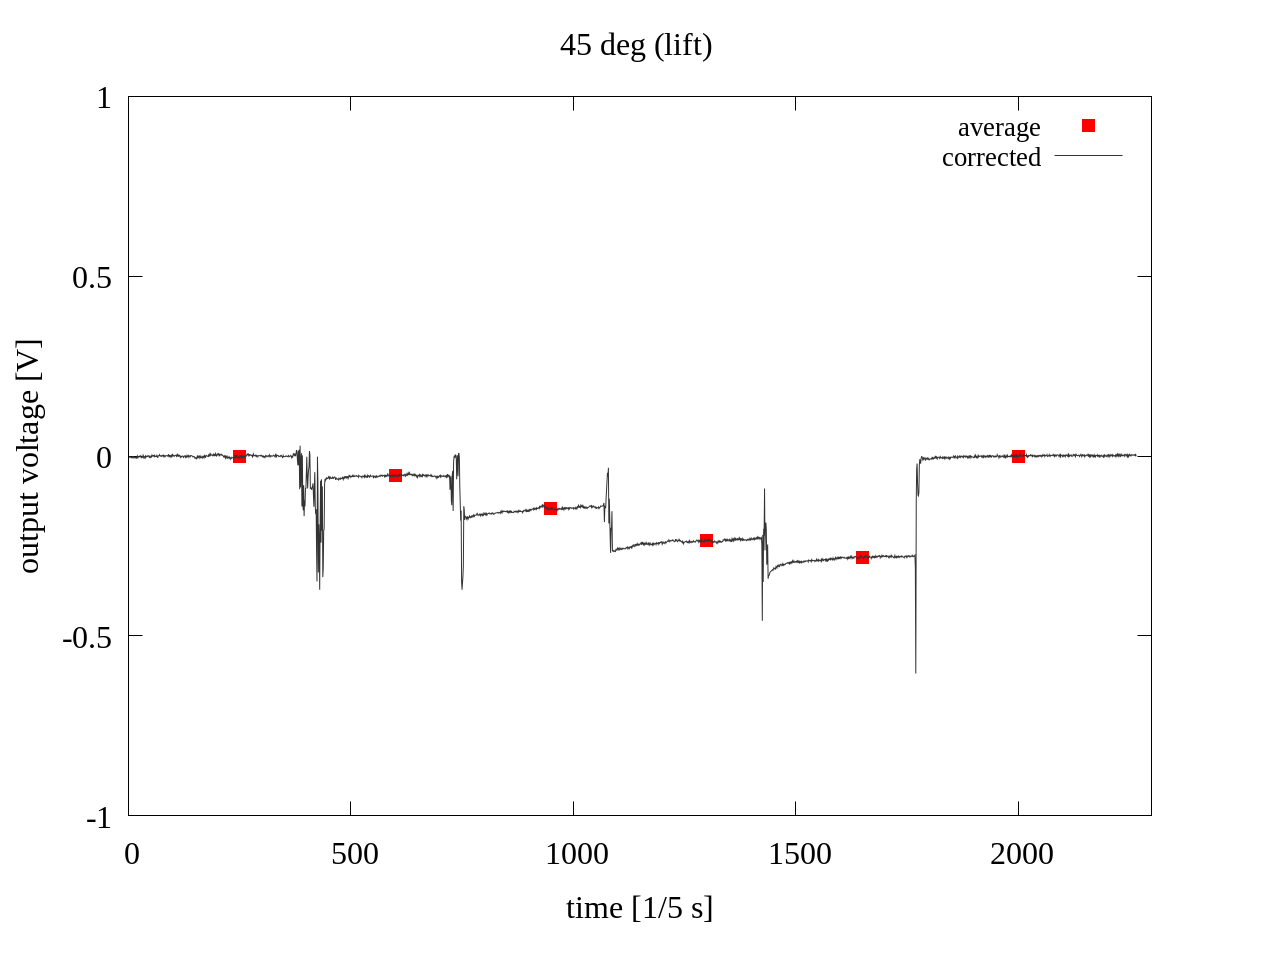
\includegraphics[width=88mm]{../images/average/45_lift_average.png}
        \caption{Average (lift)}
    \end{center}
\end{figure}

\newpage
\subsection{60 deg}
\begin{figure}[htbp]
    \footnotesize
    \begin{center}
        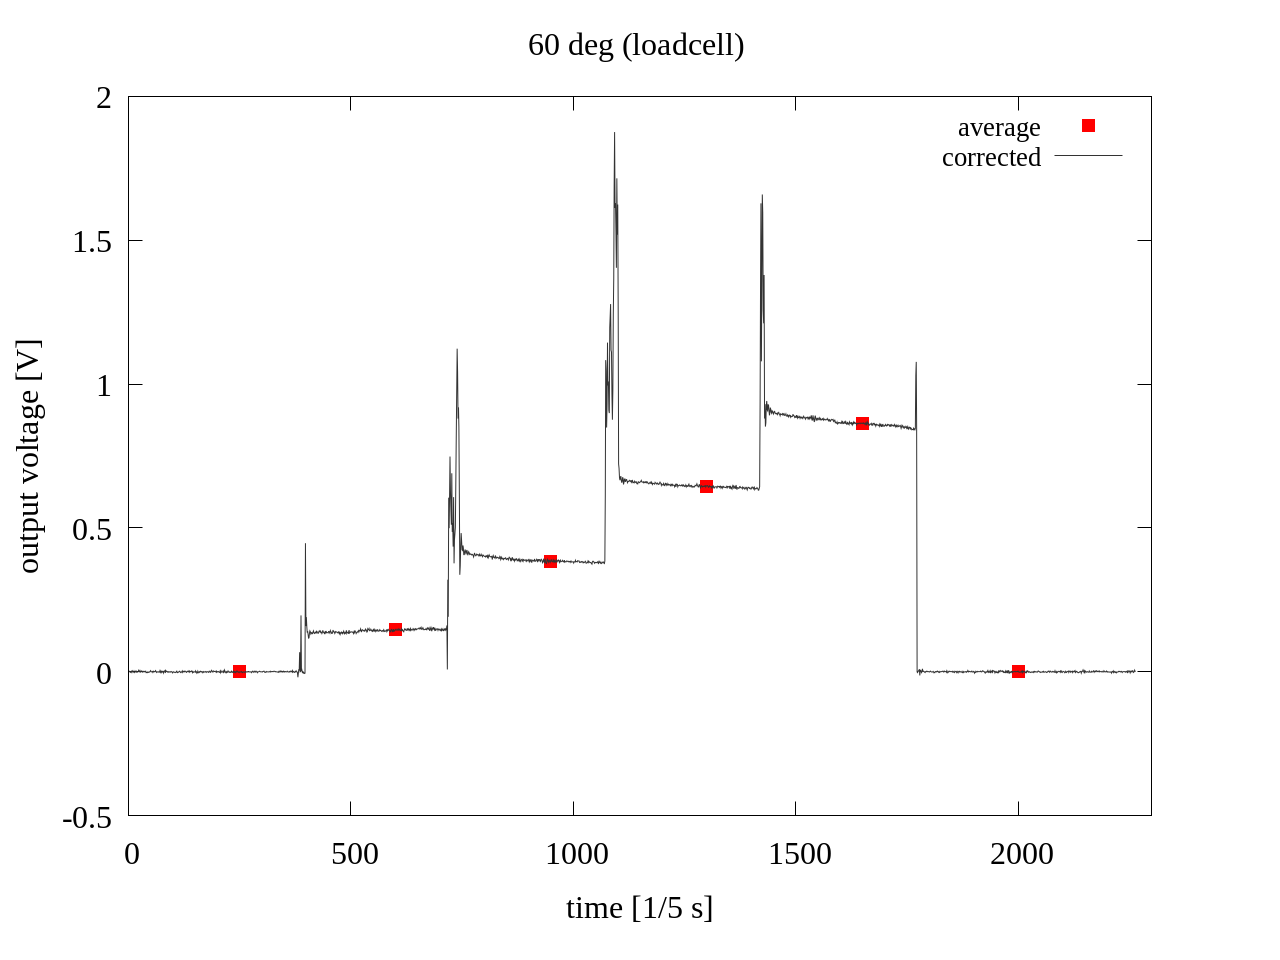
\includegraphics[width=88mm]{../images/average/60_loadcell_average.png}
        \caption{Average (loadcell)}
        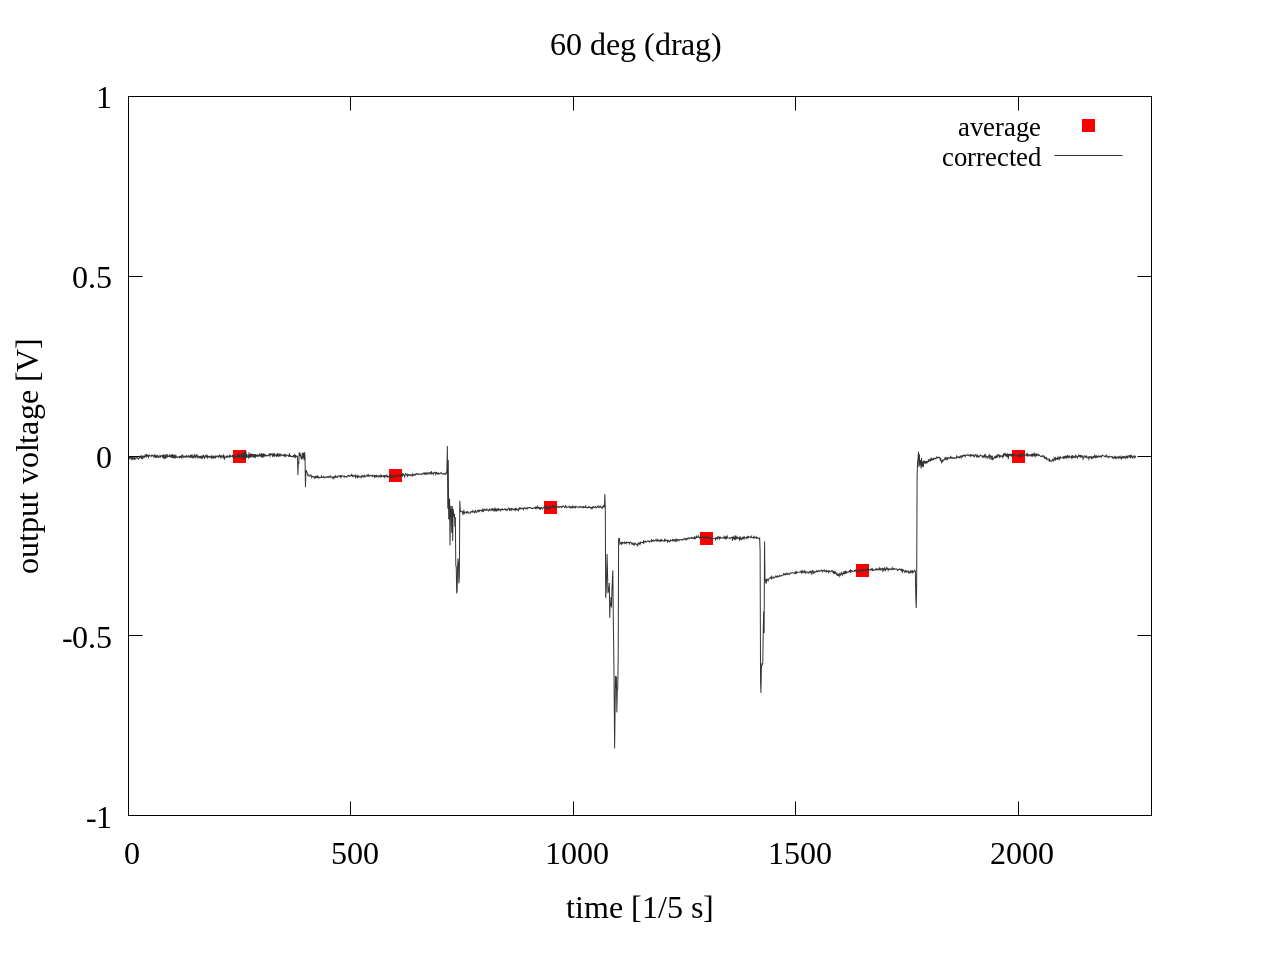
\includegraphics[width=88mm]{../images/average/60_drag_average.png}
        \caption{Average (drag)}
        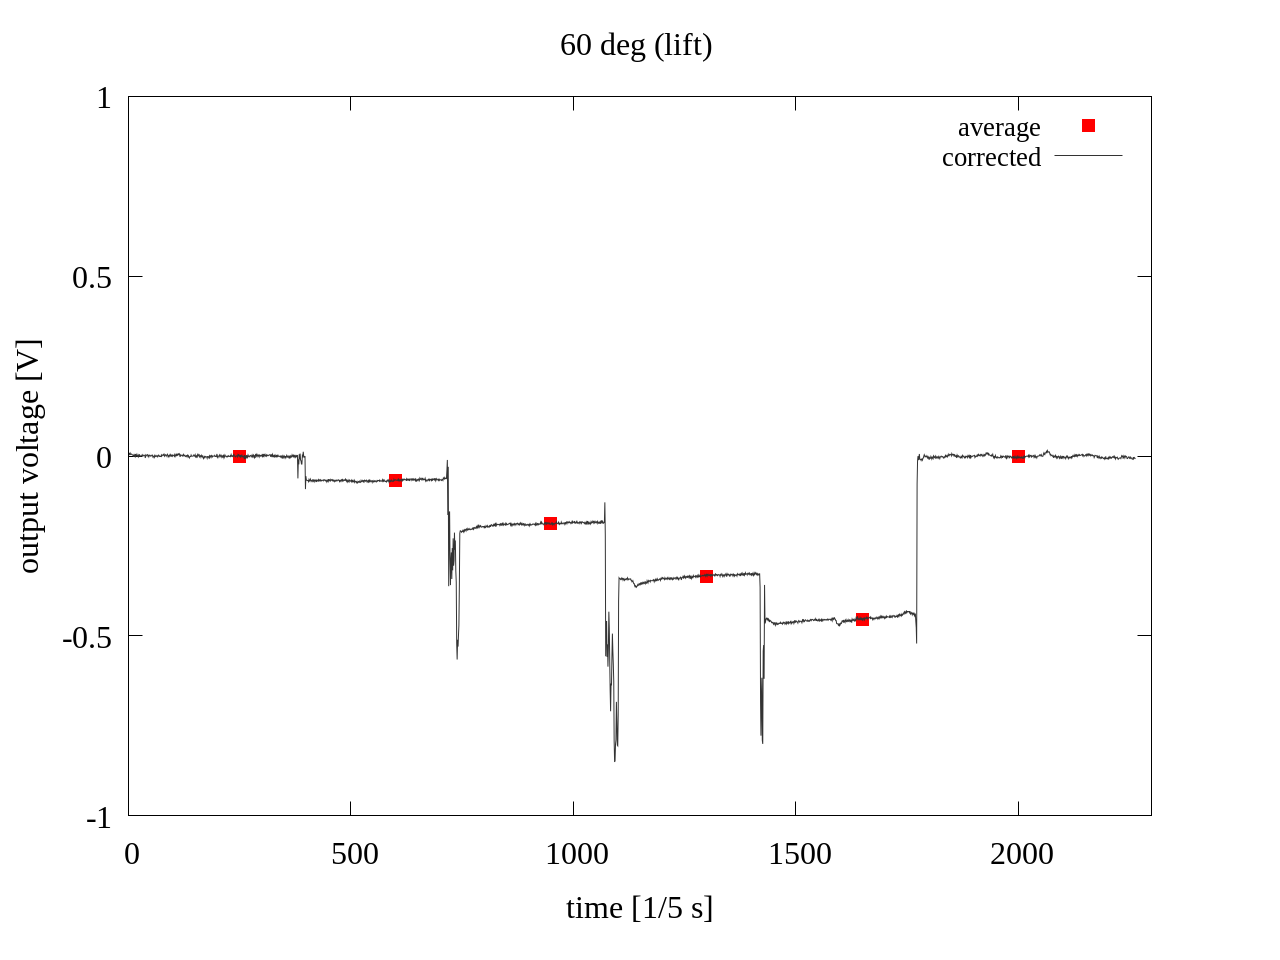
\includegraphics[width=88mm]{../images/average/60_lift_average.png}
        \caption{Average (lift)}
    \end{center}
\end{figure}

\newpage
\subsection{75 deg}
\begin{figure}[htbp]
    \footnotesize
    \begin{center}
        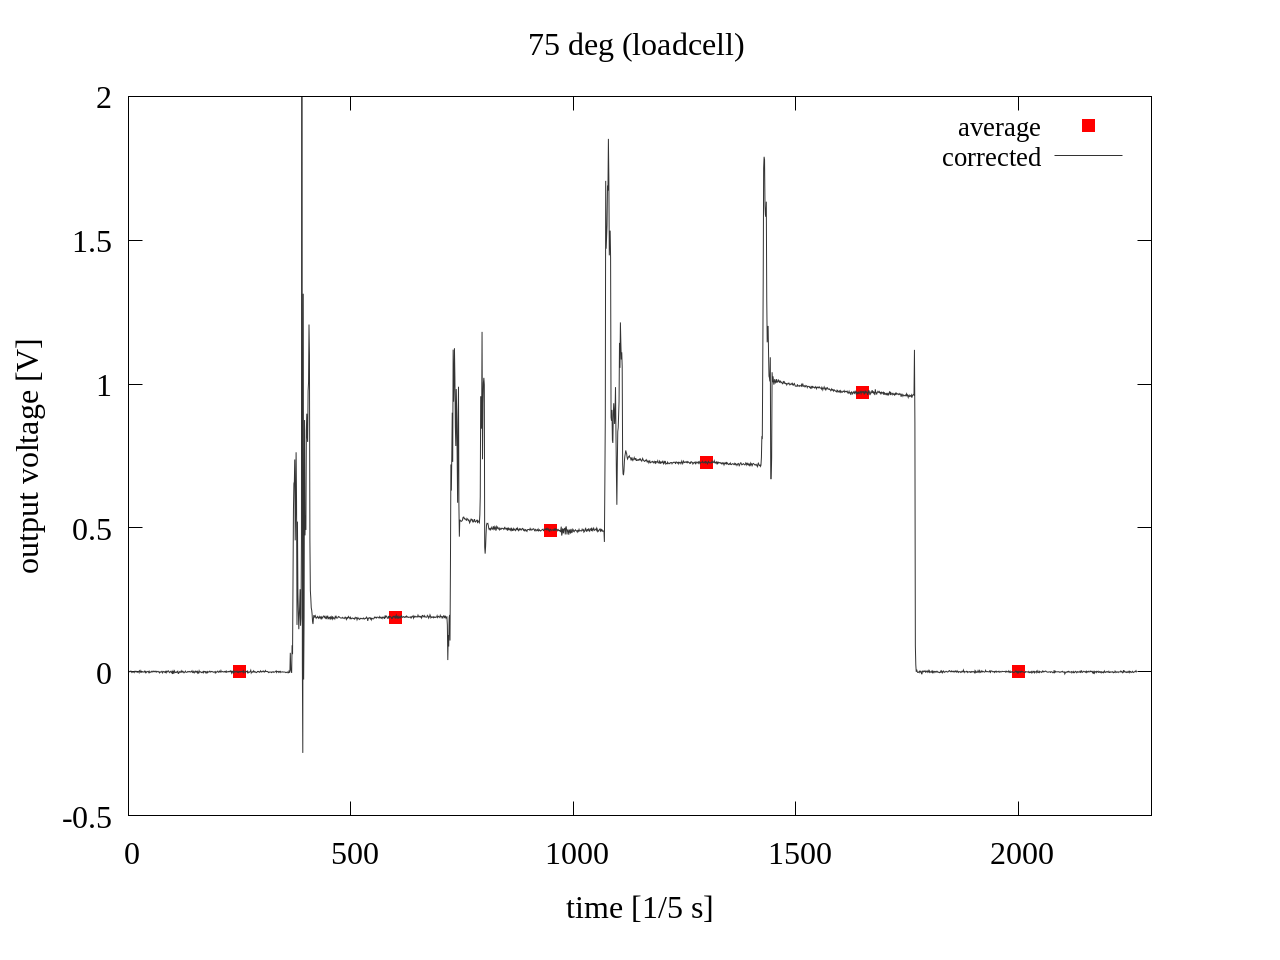
\includegraphics[width=88mm]{../images/average/75_loadcell_average.png}
        \caption{Average (loadcell)}
        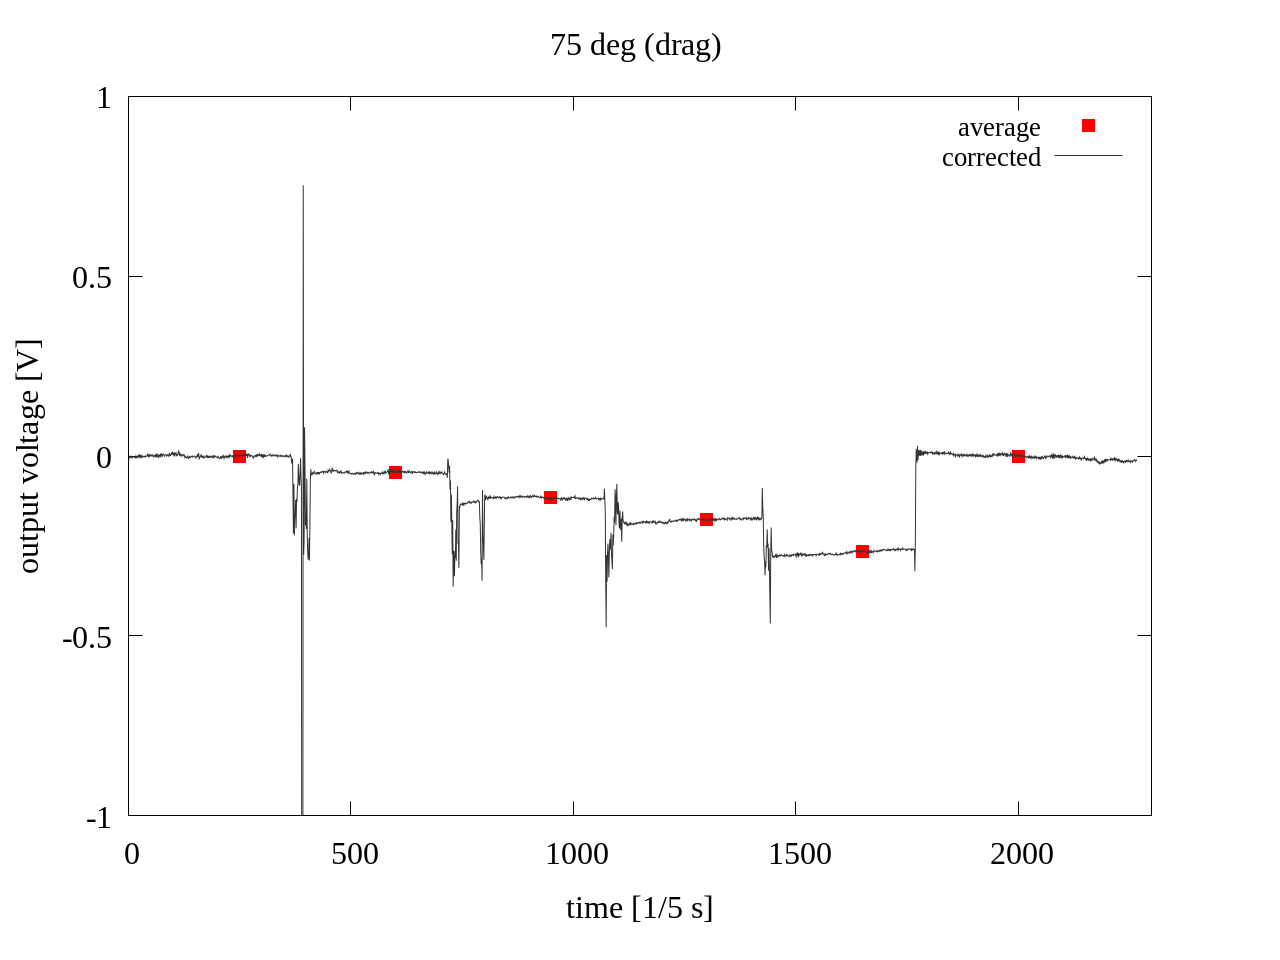
\includegraphics[width=88mm]{../images/average/75_drag_average.png}
        \caption{Average (drag)}
        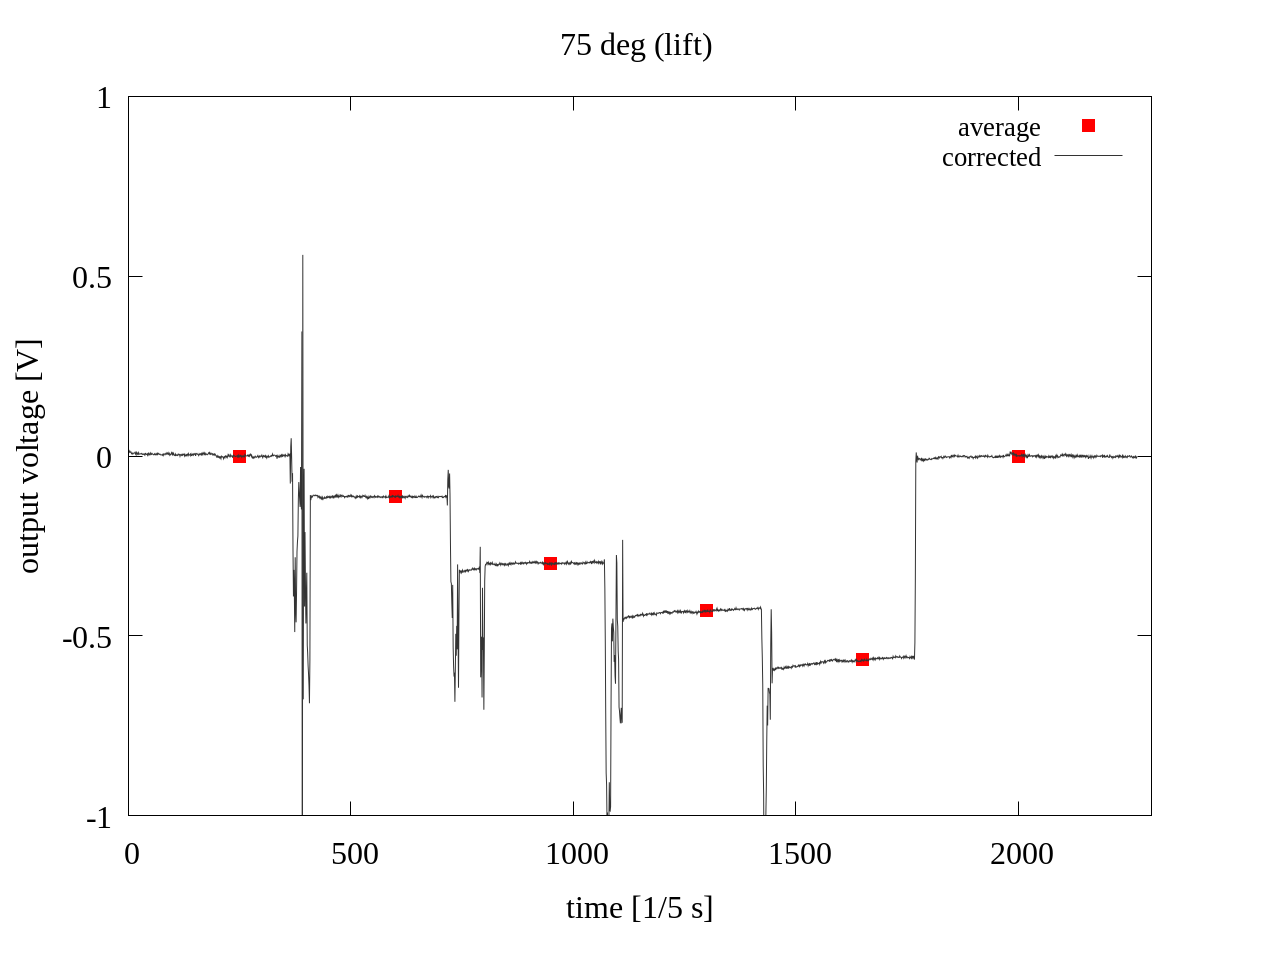
\includegraphics[width=88mm]{../images/average/75_lift_average.png}
        \caption{Average (lift)}
    \end{center}
\end{figure}

\newpage
\subsection{90 deg}
\begin{figure}[htbp]
    \footnotesize
    \begin{center}
        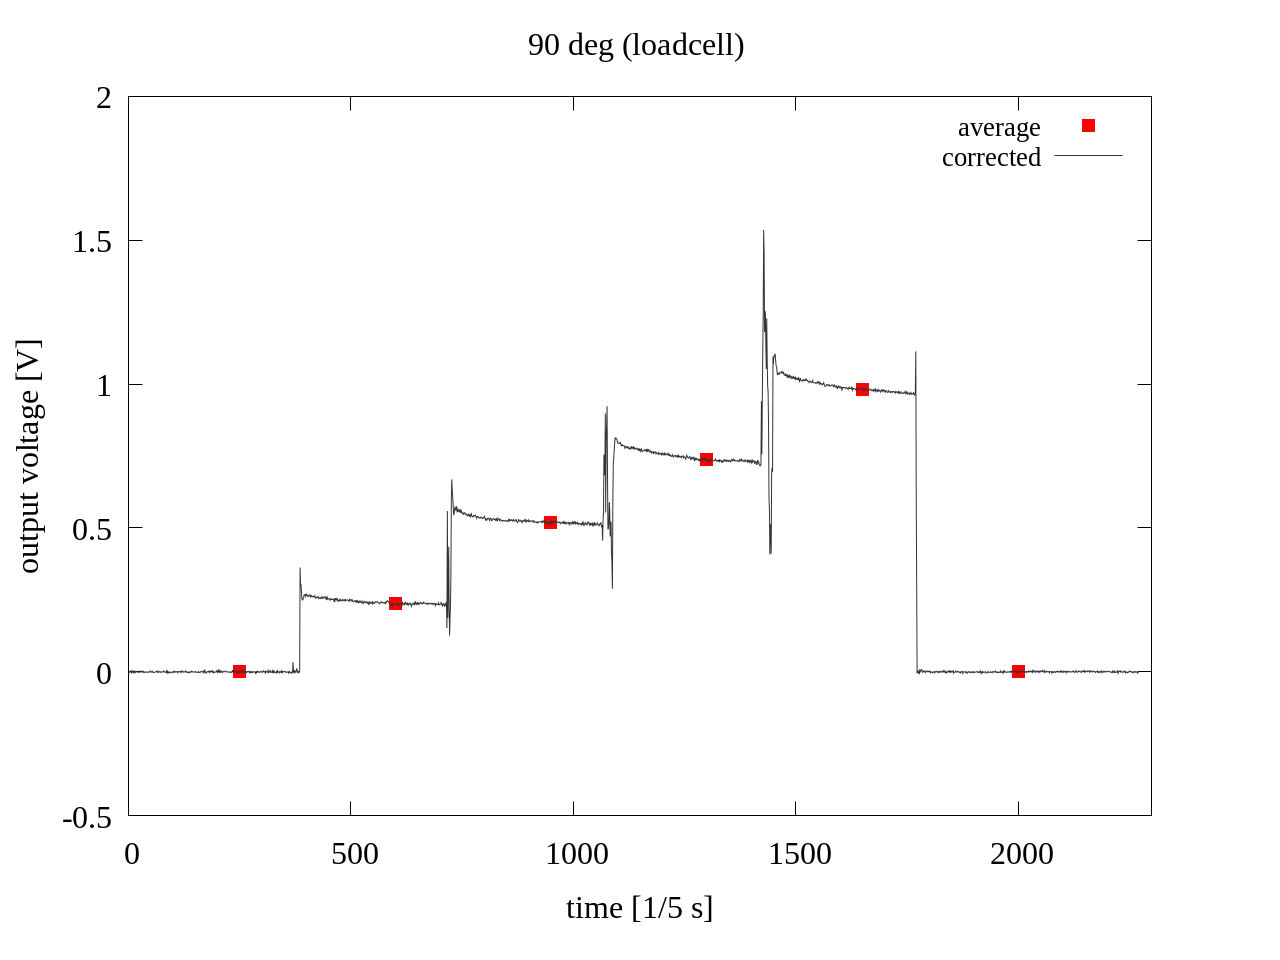
\includegraphics[width=88mm]{../images/average/90_loadcell_average.png}
        \caption{Average (loadcell)}
        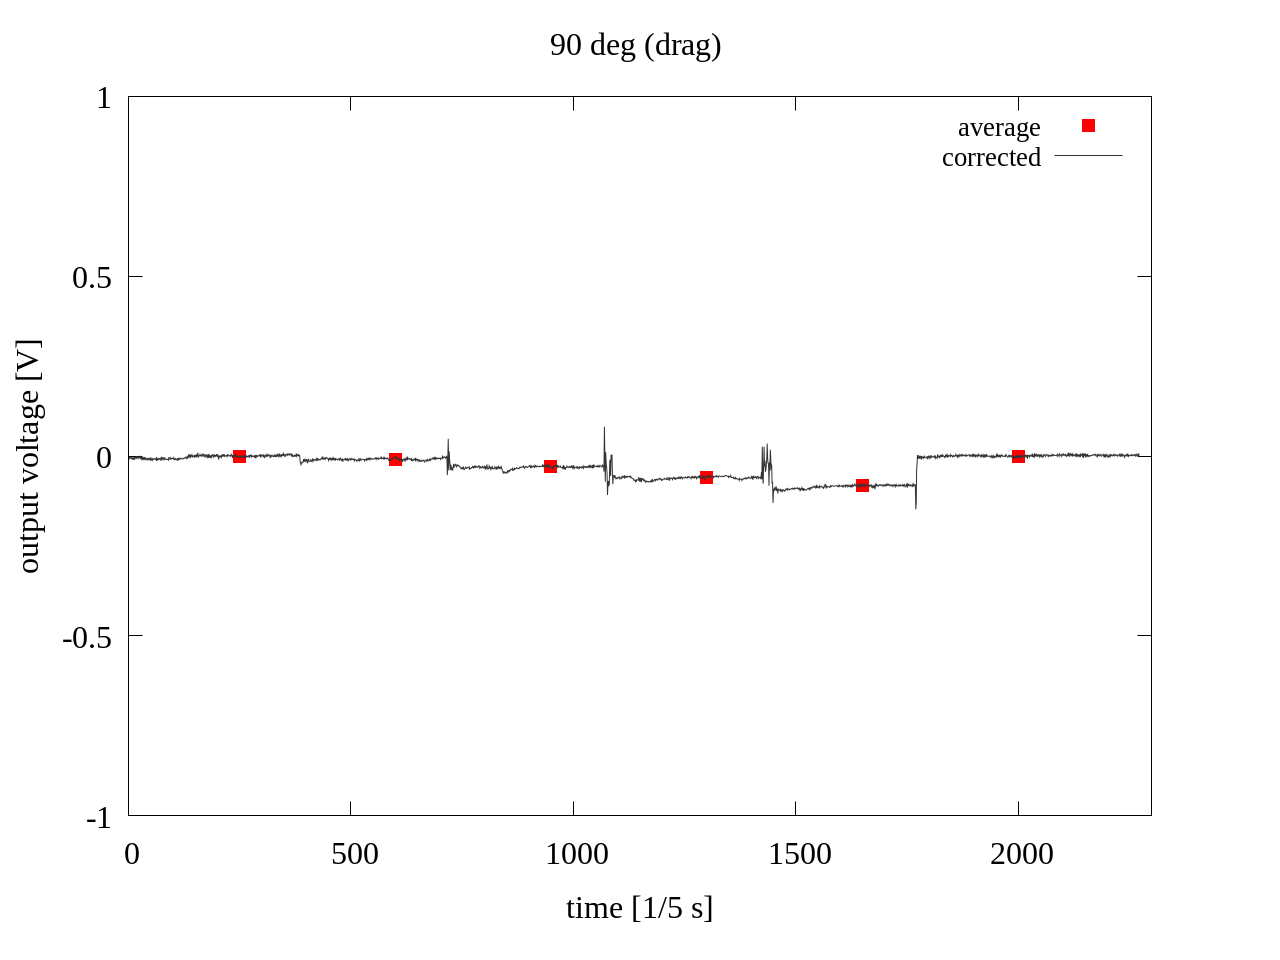
\includegraphics[width=88mm]{../images/average/90_drag_average.png}
        \caption{Average (drag)}
        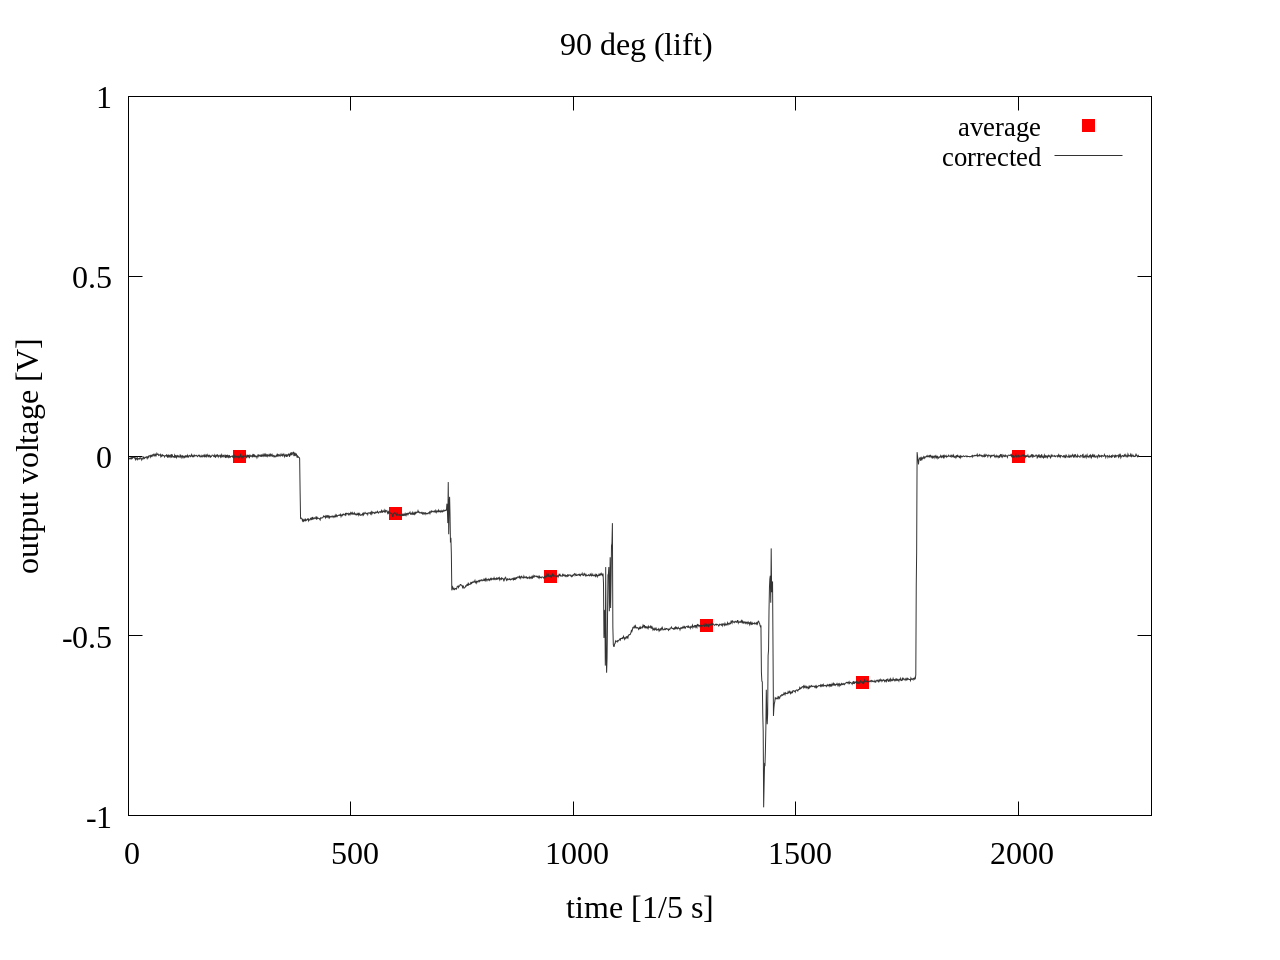
\includegraphics[width=88mm]{../images/average/90_lift_average.png}
        \caption{Average (lift)}
    \end{center}
\end{figure}

\end{document}